\documentclass{mpaper}

\usepackage{graphicx, float, multirow, booktabs, siunitx, fancyvrb, bm, subcaption}
\usepackage[format=plain, labelfont={bf},textfont=it,tableposition=above]{caption}
\usepackage[table]{xcolor}

\definecolor{lightgreen}{RGB}{166, 237, 174}
\definecolor{lightred}{RGB}{255, 189, 190}
\definecolor{lightgold}{RGB}{255, 231, 143}

\begin{document}

\title{mmFace: 3D Face Recognition using RGB and Millimetre Wave Radar}
\author{Stergious Aji}
\matricnum{2546916A}

\maketitle

\begin{abstract}
    TODO
    % According to Simon Peyton Jones, an abstract should address four key questions. First, what is the problem that this paper tackles? Second, why is this an interesting problem? Third, what is the solution this paper proposes? Finally, why is the proposed solution a good one?


\end{abstract}

% This paper outlines the standard template for a final MSci project report submission at the School of Computing Science in the University of Glasgow. In earlier years, MSci students at the School of Computing Science\footnote{\url{https://www.gla.ac.uk/computing}}, University of Glasgow, were expected to produce a full-length dissertation. Now, the requirement is for MSci students to write a paper of up to 14 pages in length, using the supplied \texttt{mpaper} \LaTeX style file.

% The precise structure of an MSci paper is not mandated, but it should probably cover in detail the following aspects of the project.
% \begin{enumerate}
% \item General description of the problem, motivation, relevance
% \item Background information, possibly including a literature survey
% \item Description of approach taken to solve the problem, including high-level design and lower-level implementation details as appropriate
% \item Evaluation, qualitative or quantitative as appropriate
% \item Conclusion, including scope for future work
% \end{enumerate}

\section{Introduction}
% Facial recognition technology is a key area of research within the field of computer vision, with widespread applications across areas such as security surveillance, forensic analysis, and human-computer interaction. Its most prominent use case lies in biometric authentication, allowing individuals access to their personal devices or restricted areas. This enables a non-invasive, hands-free approach to identity verification, removing the need to recall passwords. Furthermore, facial biometrics are naturally more accessible than other forms such as fingerprints, iris, or palm prints \cite{zhou20183d}.
Facial recognition is a key area of research within the field of computer vision, finding extensive use across areas including human-computer interaction, security surveillance, and forensic analysis. Its primary application being biometric authentication, granting individuals access to their devices or restricted zones. This enables a non-intrusive, hands-free means of identity verification, eliminating the need to memorise passwords. Additionally, facial biometrics are naturally more attainable than other modalities such as fingerprints, palm prints, or iris scans \cite{zhou20183d}.

% Since its inception in the 1960s, facial recognition systems have evolved drastically. The pioneering work by Bledsoe \cite{bledsoe1966model} first distinguished faces by comparing distances of manually annotated landmark features such as the nose, eyes, and mouth. In more recent years, the advent of deep learning has enhanced the performance and efficiency of human face classification, benefitting from the vast online repositories of face images.  Nevertheless, these systems primarily rely on images captured by RGB cameras, making them susceptible to variations in lighting and pose \cite{xu2004depth}. By incorporating depth data, which draws attention to the geometric details of the face, the effect of such environmental factors can be mitigated. Moreover, the transition to three-dimensional face recognition not only improves accuracy, but also enhances the security of biometric systems against spoofing attacks \cite{wen2015face}.
Since its inception in the 1960s, facial recognition technology has undergone significant growth. Initially pioneered by Bledsoe \cite{bledsoe1966model}, early systems distinguished faces by comparing manually annotated landmark features such as the nose, eyes, and mouth. More recently, the emergence of deep learning has amplified the performance of human face classification, benefitting from the vast online repositories of face images. Nonetheless, these systems predominantly rely on images captured by RGB cameras, leaving them vulnerable to variations in lighting and facial pose \cite{xu2004depth}. By incorporating depth data and drawing attention to the geometric details of the face, the impact of such environmental factors can be mitigated. Furthermore, the transition to three-dimensional facial recognition not only increases accuracy but also bolsters the security of biometric systems against spoofing attacks \cite{wen2015face}.


\subsection{Motivations}
% The popularity of 3D face recognition is on the rise, evidenced by its adoption in smartphones with the likes of Apple and their Face ID \cite{apple-faceid} technology. This growing demand has pushed the commercialisation of depth-sensing technology to smaller form factors, enabling it to operate efficiently in real-time on mobile devices \cite{soumya2023recent}. Face ID, in particular, has achieved a level of security that allows its integration into services like Apple Pay. However, the use of costly proprietary hardware and restrictive patents by Apple make it harder for smaller companies to adopt an equally compact and secure face recognition system.
The popularity of 3D face recognition is on the rise, evidenced by its adoption in smartphones with the likes of Apple and their Face ID \cite{apple-faceid} technology. This growing demand has pushed the commercialisation of depth-sensing technology to smaller form factors, facilitating its efficient real-time operation on mobile devices \cite{soumya2023recent}. Face ID, in particular, has garnered a level of security that enables payment authentication within services such as Apple Pay. However, Apple's use of costly proprietary hardware and restrictive patents make it harder for smaller companies to adopt an equally compact and secure face recognition system.

% Depth cameras used in this context typically employ an active acquisition method. This is where non-visible light is projected onto the face and reflected back, allowing sensors to measure and map facial features. The most common approach involves lidar cameras, emitting waves in the near-infrared (NIR) spectrum, due to their ability to capture a dense 3D map of the subject's face \cite{wang2020evolution}. However, its weakness in penetrating materials such as clothing and hair is a notable limitation. In contrast, millimetre radar waves (mmWaves) can penetrate such materials to directly reach the dermal layer of the skin \cite{vizard2006advances}, potentially offering better performance in scenarios involving facial hair, or even within challenging environmental conditions such as rain or fog.
Depth cameras used in this context typically employ an active form of acquisition. This involves projecting non-visible light onto the face, which is then reflected back, allowing sensors to measure and map facial attributes. Lidar cameras, emitting waves in the near-infrared (NIR) spectrum, are the most prevalent choice given their capacity to acquire a dense 3D map of the subject's face \cite{wang2020evolution}. However, they are often limited by their inability to penetrate thin materials such as clothing and hair. For instance, iPhone users must provide separate facial scans for scenarios involving spectacles or face masks to ensure Face ID operates effectively in all situations \cite{apple-faceid-mask}. For instance, individuals must submit separate facial scans for when they wear spectacles or face masks in order for Face ID to operate in all scenarios. In contrast, millimetre wave radar (mmWaves) can penetrate such materials and directly reach the skin's dermal layer \cite{vizard2006advances}. This could enable greater performance in scenarios involving facial hair or adverse environmental conditions such as rain or fog.

% Research into the efficacy of radar waves for 3D face recognition is relatively sparse, but recent studies show positive results \cite{hof2020face, lim2020dnn,kim2020face, pho2021radar, challa2021face}. Radar sensors are generally more cost-effective, both in terms of acquisition and computation, as they consume less power compared to NIR-based sensors. However, it is important to note the trade-off, as mmWaves tend to yield a sparser, less accurate representation in comparison. This could impact recognition performance where precision in detecting and mapping facial features is paramount. This project aims to therefore explore counter-balancing this limitation with the information gained from colour images, potentially paving the way for more resilient and versatile systems. 
Research into the efficacy of radar waves for 3D face recognition remains relatively limited, although recent studies indicate promising outcomes \cite{hof2020face, lim2020dnn, kim2020face, pho2021radar, challa2021face}. Radar sensors typically offer greater cost efficiency in terms of both acquisition and computation, as they consume less power compared to NIR-based systems. Nevertheless, it is crucial to acknowledge the trade-off, as mmWaves often result in a sparser representation. This could impact recognition performance, where the precision in detecting and mapping facial features is paramount. Thus, we aim to counter-balance this limitation with the textural information gained from colour images, potentially paving the way for more resilient and versatile systems.


\subsection{Research Contributions}
Our work explores the effectiveness of using RGB cameras in conjunction with mmWave radar sensors for 3D facial recognition. Due to the absence of suitable datasets available for this purpose, we curated our own. We use the Intel RealSense L515 RGB-D camera \cite{intel-l515} for photographing subject faces. Meanwhile, the Google's Soli \qty{60}{\GHz} radar sensor \cite{lien2016soli} is employed to gather depth information by transmitting and measuring millimetre waves reflected from the target.

We have gathered face data from \num{21} participants under various conditions encompassing diverse poses, lighting settings, and common occlusion scenarios. This comprehensive approach led to a system that demonstrates robustness to environmental factors, surpassing systems reliant solely on RGB data.

We have developed a novel face recognition model using a convolutional-based neural network architecture that is able to encode identity-specific facial characteristics into a rich multimodal representation that incorporates both RGB and mmWave radar information. We investigate different feature fusion strategies in blending the two modalities, aiming to pinpoint the most effective strategy that provides distinctive embeddings for clean identity separation. The best performing model is benchmarked against prior radar-based facial recognition systems, as well as, a base comparison to using each modality independently.

The key contributions of this paper are summarised below:
\vspace{-0.48cm}
\begin{itemize}
    \itemsep 0.08cm
    \item Compilation of a diverse face dataset comprising colour images and mmWave signatures from 21 participants. The dataset encompasses five different poses, two lighting conditions, and two occlusion scenarios.
    \item We present \texttt{mmFace}, a hybrid face recognition model that harnesses both modalities yielding a robust system capable of handling common occluding materials and nullifying 2D spoofing attempts. The model exhibits strong generalisation capabilities to unseen faces and discerns between live and fake faces effectively.
    \item An empirical analysis of seven feature-level fusion methods is conducted to determine the most optimal approach for blending RGB and mmWave facial features.
    \item Our models and evaluations are open sourced\footnote{\url{https://github.com/StergiousAji/mmFace-3D-Face-Recognition-using-RGB-and-mmWave-Radar}} to facilitate further research into small-scale, 3D face identification using mmWave technology.
\end{itemize}
\vspace{0.01cm}



\section{Background}
\subsection{mmWave Radar Technology}
Radio Detection and Ranging, or Radar, has been around for decades and plays an instrumental role in fields including space exploration, aviation, and maritime navigation. Recently, the miniaturisation of radar sensors to operate in the millimetre wave band have expanded its applicability to more small-scale domains \cite{soumya2023recent}. mmWave sensing has particularly excelled in the autonomous vehicle domain, facilitating object detection for systems such as collision warnings and adaptive cruise control \cite{dfrobot}. This is primarily due to its edge over traditional lidar cameras, specifically in its resilience to atmospheric conditions such as dust, smoke, fog, and rain \cite{cadenceblog2022}. This penetrative power of mmWaves make it a promising candidate for reliable facial recognition in uncertain, real-world scenarios. 

Another notable example is Google's integration of their Soli sensor into the Pixel 4 smartphones for motion detection and gesture recognition \cite{googleblog2020}. However, the sensor's potential application to face recognition remains unexplored, presenting a unique research opportunity. Consequently, this is the sensor we use to capture mmWave face signatures during our data collection procedure. A key driving factor for this choice is the Soli's miniature form factor of just \qty{6.5}{\mm} $\times$ \qty{5.0}{\mm}, and its use of Frequency Modulated Continuous Wave (FMCW) technology. This is proven to offer superior range resolution in comparison to other modulation techniques thanks to its high pulse compression \cite{mahafza2005radar}, a vital aspect for extracting accurate facial features. Furthermore, The Soli chip has a relatively low power consumption due to the fact that it sends 16 chirps every burst at a pulse-repetition frequency of \qty{2}{\kHz}, after which it halts transmission until the next burst of chirps \cite{hayashi2021radarnet, mitchell2023mmsense}. Each burst is transmitted at rate of \qty{25}{\Hz} giving an overall transmission duty cycle of 2\%. This effectively means that the radar chip remains inactive during the majority of its operation, saving a lot of power for small-scale mobile applications.
% However, it is important to note the trade-off, as mmWaves tend to have a lower accuracy in comparison. This could impact face recognition performance where precision in detecting and mapping facial features is paramount. This project will therefore explore counter-balancing this limitation with the information gained from RGB images, potentially paving the way for more resilient and versatile systems.

\vspace{0.05cm}
\subsection{Related Work}
% The use of millimetre waves for face identification is a relatively new research field, spurred by the recent commercialisation of radar sensor technology. One of the earliest studies found to investigate human identification using mmWaves can be traced back to 2019, conducted by Zhao et al. \cite{zhao2019mid}. Although this paper focuses on classifying subjects by their gait and body shape rather than facial features, it demonstrates the ability of mmWaves to encapsulate the subtle idiosyncrasies among individuals. These nuanced differences are vital for learning models to effectively differentiate between unique subjects, leading to high classification accuracies.
The use of millimetre waves for face identification is a relatively new avenue of research, fuelled by the recent commercialisation of radar sensor technology. One of the earliest studies delving into human identification using mmWaves dates back to 2019, conducted by Zhao et al. \cite{zhao2019mid}. While this paper primarily examines the classification of subjects based on their gait and body shape rather than facial features, it underscores the capacity of mmWaves to capture the subtle idiosyncrasies among individuals. These nuanced differences are crucial for machine learning models to accurately distinguish between unique subjects, thereby yielding high class separations.

% Following this, Hof et al. \cite{hof2020face} proposed an Autoencoder that can distinguish human faces captured by an 802.11ad/y networking chipset operating at a centre frequency, $f_c$, of 60 GHz. The Autoencoder is able to encode mmWave face signatures of over 200 individuals with enough separation to distinguish between positive and negative instances by measuring their Mean Squared Error (MSE) against reference facial embeddings. The study conducted an extensive data collection process, capturing face scans of 206 participants comprising various genders and ages, in five different poses: frontal, as well as, $15^\circ$ and $25^\circ$ head rotations to the left and right. This collection was subsequently made available through an IEEE Data Port \cite{mmwavefacedata}. While this dataset encapsulates faces from a wide range of people, including some with beards and spectacles, it lacks representation of other common occlusion scenarios like head accessories, that our project aims to explore. Moreover, the study utilised a larger sensor containing a total of 1024 transmit-receiver antenna pairs, found to capture redundant information. This is in contrast to the compact Soli chip, intended to work within a smartphone. The study simulated the effect of reducing the antenna count to 10, markedly decreasing the distinctiveness of facial signatures. Promisingly, increasing the number of neurons in their Neural Network and an additional hidden layer could compensate for this reduction, maintaining high accuracy.
The following year, Hof et al. \cite{hof2020face} introduces an autoencoder capable of recognising human faces captured by an 802.11ad/y networking chipset operating at a \qty{60}{\GHz} centre frequency ($f_c$). This autoencoder effectively encodes mmWave face signatures with sufficient distinction to discriminate between positive and negative instances based on their Mean Squared Error (MSE) against reference embeddings. The study involved an extensive data collection effort, capturing face scans of 206 participants of varying genders and ages, across five different poses: frontal, as well as head rotations of $15^\circ$ and $25^\circ$ to the left and right. This dataset was subsequently made available through an IEEE Data Port \cite{mmwavefacedata}. While this collection encompasses a wide range of faces, including some individuals with spectacles and beards and, it lacks representation of other common occlusion scenarios, such as head accessories, which our project aims to explore. Additionally, the study utilised a larger sensor with a total of 1024 transmit-receive antenna pairs, noted to capture redundant information. This contrasts with the compact Soli chip designed for integration within smartphones. The study simulated the impact of reducing the antenna count to 10, resulting in a significant decrease in the distinctiveness of facial signatures. Encouragingly, increasing the number of neurons in their Neural Network and adding an extra hidden layer could compensate for this loss.

Lim et al. \cite{lim2020dnn} proposes a deep neural network with a more traditional Multi-Layer Perceptron (MLP) approach where every layer is fully connected to adjacent ones. The study utilised a small-scale, \qty{61}{\GHz} FMCW radar sensor developed by bitsensing Inc. \cite{bitsensing2020bts60}, comparable to the Soli with a single transmit and three receiver antennas. The model attained a mean classification accuracy of 92\% across eight subjects, surpassing the performance of both, a Support Vector Machine (SVM), and a tree-based Ensemble Learning approach trained on the same face signatures. It is important to note the relatively small-sized dataset used to train the model, raising concerns about potential overfitting as the data is not representative enough. The paper provides limited details on the data collection methodology used, only mentioning that the distances ranged from \qty{30}{\cm} to \qty{50}{\cm}. It can be assumed then that the study likely focussed on frontal poses without any occlusions for all eight subjects. 
% The research also explored the impact of using a single receiving antenna, which resulted in a reduced accuracy of 73.7\%. This finding is in line with Hof et al.'s \cite{hof2020face} observation that an increased number of receiving antennas can enhance classification accuracy by the ability to capture more nuanced facial features.

% During the same period, Kim et al. \cite{kim2020face} conducted research using an identical sensor from bitsensing Inc., featuring a range resolution of 2.5 cm. Their study introduces a CNN model comprising three convolutional layers and three fully connected layers. The radar data underwent heavy preprocessing to transform it into a more image-like format suitable for the CNN model. With a data split of 70\%/15\%/15\% for training, validation, and testing, the model achieved an average classification accuracy of 98.7\% on a limited dataset of only three individuals. Interestingly, the study also examined the impact of wearing cotton masks. The results showed a minimal drop in average classification accuracy by 0.9\%, which is encouraging for the objectives of our project. However, these findings are to be taken with caution due to the small size of the dataset. It remains unclear whether this level of performance would hold consistently across a larger group of subjects with more varied occlusions.
During the same time frame, Kim et al. \cite{kim2020face} conducted research utilising an identical sensor from bitsensing Inc., which boasted a range resolution of \qty{2.5}{\cm}. Their study introduces a Convolutional Neural Network (CNN) model consisting of three convolutional layers and three fully connected layers. The radar data underwent extensive preprocessing to convert it into a format more akin to images, suitable for the CNN. With a data split of 70\%/15\%/15\% for training, validation, and testing, the model achieved an average classification accuracy of 98.7\% on a limited dataset of only three individuals. Notably, the study also investigated the impact of wearing cotton masks. The results indicated a negligible decrease in average classification accuracy by 0.9\%, which bodes well for the goals of our project. Nonetheless, it is important to approach these findings with caution due to the small dataset size. It remains uncertain whether this level of performance would hold consistently across a larger group of subjects with more varied occlusions.

Pho et al. \cite{pho2021radar} adopts a One-Shot Learning approach to the problem. This is where the model is trained with a single or only a few labelled instances, beneficial when there is a lack of training samples available. The proposed method constitutes a Siamese structure of two identical CNNs with shared parameters, mapping the input radar signals into latent space. During both training and testing phases, a distance metric between the outputs of the networks is used to assess the similarity between face inputs. Specifically trained for binary classification, the model receives pairs of face signatures from either the same or different individuals. The same bitsensing Inc. BTS60 chipset, used by Lim et al. and Kim et al. \cite{lim2020dnn, kim2020face}, is employed to capture 500 frames of the faces of eight participants. An average classification of 97.6\% was achieved, an improvement over the previous deep MLP model by Lim et al. involving the same number of people. t-Stochastic Neighbour Embedding (t-SNE) \cite{van2008visualizing} is then applied for dimensionality reduction. The resulting visualisations demonstrate that the one-shot Siamese network effectively separates each individual's face into exclusive regions, simplifying the classification task. Although a small dataset is used, only encompassing frontal poses with no occlusion settings, the proposed method is well documented and is likely robust against larger datasets.

Challa et al. \cite{challa2021face} employs two different machine learning models on the dataset provided via the IEEE port \cite{mmwavefacedata}. Their approach began with CNN-based autoencoders, followed by a Random Forest Ensemble Learning approach. A total of nine autoencoders were built, each tailored to different frame rates, focusing on compressing and reconstructing the original data from its latent form. The autoencoders were trained using randomly selected data samples from a subset of 186 face scans. The flattened and labelled outputs were then used to train and test nine discrete Random Forest models using identical hyperparameters, as recommended by the Sci-kit library. This methodology yields impressive results, achieving an average classification accuracy of 99.98\% using all 1400 frames per individual. Even when reducing the number of frames to 70 per person, the model maintained a high accuracy of 97.1\%. The paper presents an approach that is unique in comparison to the rest of the papers tackling this subject, showcasing an efficient model that is able to be deployed on mobile chips.

% The research in this area exclusively focuses on utilising data from radar sensors, largely driven by concerns of privacy preservation. However, a significant limitation of this approach is the required duration for capturing an accurate facial scan. The sensor needs to operate for several seconds, typically in the range between 10 and 15 seconds, in order to obtain a detailed scan. Such a time frame is impractical in real-world situations, as it necessitates the subject to remain motionless for a prolonged period. Up to this point, no study was found to explore the potential benefits of combining radar signatures with corresponding RGB data to enhance facial recognition capabilities. Given the high performance of existing deep learning models using RGB images alone, such as InsightFace \cite{deng2018arcface}, integrating these models with mmWave radar data presents a promising avenue. This combination could accelerate face acquisition time, while leveraging the advantages of mmWaves in terms of their robustness to lighting variations and occlusions.
Research in this domain focuses exclusively on utilising data from radar sensors, largely driven by concerns surrounding privacy preservation. However, a significant drawback of this approach lies in the extended duration required to capture an accurate facial scan. The sensor typically needs to operate for several seconds, ranging between 10 and 15 seconds, to obtain a detailed scan. Such a time frame proves impractical in real-world scenarios, as it requires the subject to remain motionless for a prolonged period. Thus far, no study has explored the potential benefits of combining radar signatures with corresponding RGB data to enhance facial recognition capabilities. Given the high performance of existing deep learning models using RGB images alone, such as InsightFace \cite{deng2018arcface}, integrating them with mmWave radar data presents a promising avenue. This could expedite face acquisition time while capitalising on the advantages of mmWaves for environments where optical methods falter.


\subsection{InsightFace}
\label{background:insightface}
In the evolving field of face recognition, deep CNNs have emerged as a dominant approach due to their ability to automatically extract discriminative facial features from images. One significant advancement in this area is the InsightFace toolkit, implementing algorithms designed to address the intricacies of face analysis and recognition. Key works include the preliminary ArcFace model, introduced by Deng et al. \cite{deng2018arcface}, alongside the robust Face Alignment model by Gho et al. \cite{guo2018stacked}. ArcFace employs a novel Additive Angular Margin Loss to maximise class separability, further enhancing the discriminative power in mapping face images to feature embeddings. However, this method was found to face challenges with label noise, requiring the ``cleaning'' of many real-world images sourced from the web. To address this, further progress was made with the Sub-center ArcFace model \cite{deng2020subcenter}, introducing the concept of sub-classes to boost resilience against intra-class variations and label noise. It achieved state-of-the-art performance on many widely used benchmark datasets such as the Labeled Faces in the Wild (LFW) \cite{huang2008labeled} and the YouTube Faces (YTF) datasets \cite{wolf2011face}. The integration of pretrained models offered by InsightFace into our system enables us to concentrate efforts on enhancing the performance of our model's ability in extracting 3D structural information from mmWave face signatures. 
% By fusing the depth and contour detection capabilities of mmWave radar with the rich, textural features gathered by ArcFace from RGB images, the system has the potential to attain improved accuracy and robustness. This approach is particularly promising in environments where conventional optical methods falter.


\subsection{Multimodal Data Fusion Methods}
Multimodality, as defined by Lahat et al. \cite{lahat2015multimodal}, refers to the use and analysis of multiple types of data, potentially arriving from multiple sensors. The idea is to extract and blend salient information gathered by each sensor. The integration of this diverse data lead to outputs with richer representations than what could be achieved by the individual modalities alone. 
% We hypothesise that coupling the textural information from colour images with the depth gathered by the radar sensor could greatly improve class separation, and subsequently, face recognition performance.

% A common technique involves fusing the multiple data modalities before feeding them into a learning model, referred to as \textbf{Early Fusion}, or \textbf{Data-level Fusion}. It includes combining data by removing correlations between sensors or fusing data in a common, lower-dimensional space \cite{khaleghi2013multisensor}. Techniques such as Principal Component Analysis (PCA) and Canonical Correlation Analysis (CCA) are commonly employed for this purpose. One key issue with applying early fusion is ensuring synchronisation between the RGB and radar frames, which is difficult due to their significantly different sampling rates. Furthermore, the continuous mmWave signals must be effectively discretised to match the form of the RGB data. A major disadvantage of early fusion is the potential to squash critical information present within each individual modality, impacting the training efficacy.
One common strategy involves merging multiple data modalities before feeding them into a learning model, known as \textbf{Early Fusion} or \textbf{Data-level Fusion}. This technique entails combining data by eliminating correlations between sensors or fusing data in a common, lower-dimensional space \cite{khaleghi2013multisensor}. Methods like Principal Component Analysis (PCA) and Canonical Correlation Analysis (CCA) are frequently utilised for this purpose. However, a significant issue with early fusion is ensuring synchronisation between the RGB and radar frames, which is challenging due to their notably different sampling rates. Moreover, the continuous mmWave signals must be discretised to align with the format of the RGB data. An inherent drawback of early fusion is the potential to squash crucial information present within each individual modality, thereby impacting training effectiveness.

% \textbf{Late Fusion}, or \textbf{Decision-level Fusion}, operates by independently processing different data sources through separate models and then fusing them at the decision-making stage. A standard approach involves taking a weighted average of the separate predictions, providing a way to minimise or maximise the influence of specific modalities \cite{pawlowski2023effective}. Late fusion is often simpler and more flexible, and it can be effective when dealing with extremely dissimilar data sources either in terms of sampling rate, dimensionality, or unit of measurement. Additionally, late fusion often yields better performance since errors from multiple models are dealt with independently.
\textbf{Late Fusion}, or \textbf{Decision-level Fusion}, operates by independently processing distinct data sources through separate models and then integrating them at the decision-making stage. A common approach involves calculating a weighted average of the separate predictions, allowing a way to regulate the influence of specific modalities \cite{pawlowski2023effective}. Late fusion is often simpler and more adaptable, proving effective when dealing with highly dissimilar data sources in terms of sampling rate, dimensionality, or units of measurement. Furthermore, late fusion often yields better performance since errors from multiple models are managed independently.

% \textbf{Intermediate Fusion} or \textbf{Feature-level Fusion} is based on neural network architectures and involves the idea of combining different modalities within the feature space where there is a higher level of abstraction of the raw data. This can be as straightforward as a simple concatenation of the individual latent embeddings, or as complex as using Autoencoders for non-linear feature fusion as demonstrated by Charte et al. \cite{charte2018practical}. This approach offers greater versatility than early and late fusions, as it allows for the integration of features at various depths within the neural network. However, it can lead to challenges such as a risk of overfitting or a failure in learning relationships between the different modalities.
\textbf{Intermediate Fusion}, or \textbf{Feature-level Fusion}, is rooted in neural network architectures and revolves around the concept of combining different modalities within the feature space where there is a higher level of abstraction of the raw data. This can range from a basic concatenation of the individual latent embeddings to employing autoencoders for non-linear feature fusion, as demonstrated by Charte et al. \cite{charte2018practical}. This approach offers greater versatility than early and late fusions since it allows for the integration of features at various depths within the neural network. However, it can pose challenges such as the risk of overfitting or difficulty in learning relationships between the different modalities.

% Each data fusion technique comes with its own set of challenges and considerations, necessitating experimentation to determine the most effective way to merge the RGB and mmWave signatures. A variant of late, feature-level fusion where the embeddings from the last layers of each model are combined is what was chosen. It would be challenging to attempt early fusion due to the substantial differences between the two modalities. Such integration would likely require heavy preprocessing of the radar data, potentially involving its conversion into a depth image.
Each data fusion technique presents its own set of considerations, necessitating experimentation to determine the most effective approach to merging RGB and mmWave signatures. A variant of late, feature-level fusion, where the embeddings from the final layers of each model are combined, was chosen as the most feasible. 
% It would be challenging to attempt early fusion due to the substantial differences between the two modalities. Such integration would likely require heavy preprocessing of the radar data, potentially involving its conversion into a depth image.



\section{Methodology}
\subsection{Data Acquisition}
% Following a thorough research of the field, the next steps involved designing and conducting the data acquisition process necessary to train our proposed model with. These experiments required careful planning since the data collected here directly determines the effectiveness of the resulting model. As found in the related works, it is vital to compile multiple poses in order for the model to learn a comprehensive 3D scan of the individual's face. Furthermore, it induces pose-invariance into the system, accommodating real-world use cases where individuals may not always present an exact frontal pose to the face recognition system. Most studies concentrate on azimuth variations since a person is less likely to tilt or pitch their head by a significant angle in comparison to left and right rotations of the face. For this reason, we will similarly focus on head rotations around the yaw axis. We plan to record facial poses at $0^\circ$, $30^\circ$ and $45^\circ$ azimuth relative to the sensors.
Following a comprehensive research of the field, the subsequent steps involved planning and executing the data acquisition process required to train our proposed model. These experiments necessitated meticulous planning as the collected data directly determines the efficacy of the final model. As demonstrated by previous studies, it is crucial to compile multiple poses to enable the model to learn a complete 3D scan of the individual's face. Moreover, incorporating pose-invariance into the system is essential to accommodate real-world scenarios where individuals may not always present an exact frontal pose to the facial recognition system. Most studies focus on azimuth variations since individuals are less likely to tilt or pitch their heads by a significant amount. We similarly concentrated on head rotations around the yaw axis, deciding to capture facial poses at $0^\circ$, $30^\circ$, and $45^\circ$ azimuth relative to the sensors.

% Since this experiment aims to explore the benefits of mmWave sensors in the context of face recognition, two different lighting conditions are incorporated in our data collection experiments. Namely, regular and dim lighting scenarios. We hypothesise that the mmWave face signatures would be unaffected by environmental lighting due to the sensor using its own active illumination of the target face, unlike the RGB camera. Therefore, if the system is able to demonstrate higher accuracy utilising both modalities as opposed to relying solely on RGB data, it would decisively indicate that mmWaves offer resilience against varying lighting conditions.
Given that the experiment's objective is to explore the advantages of mmWave sensors for face recognition, we included two distinct lighting conditions in our data collection trials: standard and low-light environments. Our hypothesis is that mmWave face signatures remain unaffected by ambient lighting since the sensor employs its own active illumination on the target face, unlike the RGB camera. Hence, if the system can achieve higher accuracy by incorporating both modalities rather than relying solely on colour, it would strongly indicate that mmWaves provide robustness against diverse lighting conditions.

% Finally, we investigate the penetrative power of mmWaves to directly reach the skin through cloth and hair by injecting common occlusion scenarios into our experiments. It would be beneficial for facial recognition systems to be inherently robust against typical obstructions such as glasses, hats, masks and so on. Currently, users would be required to remove such accessories for systems to accurately identify and grant them access to particular devices or areas. With mmWaves, we hypothesise that this may not be needed since facial features could be captured regardless. This could greatly benefit security surveillance where individuals deliberately obscure their faces in order to hide their identities. In our experiment, we capture scenarios both with and without occlusion. Since cotton masks have already been explored by Kim et al. \cite{kim2020face}, other common items like hats, sunglasses, and scarves are used to mirror day-to-day scenarios.
Finally, we delve into assessing the permeating capability of mmWaves to directly reach the skin through fabric and hair by injecting typical occlusion scenarios into our experiments. It is advantageous for facial recognition systems to inherently withstand common obstructions such as glasses, hats, masks, and so on. Presently, users often need to remove such accessories for systems to accurately identify and grant access to specific devices or areas. With mmWaves, we speculate that this may not be required as facial features could be captured regardless. This could benefit security surveillance, especially in situations where individuals deliberately obscure their faces to conceal their identities. In our experiment, we capture scenarios both with and without occlusion. While cotton masks have been previously explored by Kim et al. \cite{kim2020face}, we incorporate other typical items such as sunglasses, hats, and scarves to mirror day-to-day use cases.

% On top of investigating environmental invariances, our research seeks to determine the least amount of radar data necessary to still yield easily separable facial embeddings. Previous studies were observed to record between 200 and 2,000 total frames which, depending on the sampling rate, requires running the sensor for eight to a maximum of 80 seconds for each scenario. This is due to the lower accuracy of mmWaves demanding a longer exposure to provide a dense enough representation. Nevertheless, requiring an individual to keep their face still for over three seconds is impractical in real-world applications. Our approach, which integrates RGB data, may reduce the need for prolonged radar frame capture. Consequently, in our experiments, we will collect 10 RGB frames and a maximum of 250 frames worth of mmWave bursts, equivalent to operating the Google Soli sensor for 10 seconds at a 25 Hz sampling rate. This approach will provide ample data to assess the minimum number of mmWave frames needed for effective identification. 

To ensure a diverse range of facial data, we recruited 21 participants within the limited time frame of the project. Adhering to ethical standards regarding sensitive personal information, our participant pool consists of male and female university students and faculty in the age range 18--35 years. A total of 15 scenarios are captured for each participant at a distance of \qty{20}{\cm} from the sensors. Each time the sensors are run for 10 seconds, totalling 150 RGB frames and 3,750 mmWave frames per person. On top of this, scans of printed faces are also collected in order to train the model to detect facial authenticity as well as its identity. This was restricted to the three frontal poses for each participant, mirroring common spoofing tactics, providing another 30 RGB frames and 225 mmWave frames per fake instance.

A close-up of the equipment setup used can be observed in Figure \ref{fig:equipment} showing the Intel Realsense RGB-D camera and the green Soli chip mounted side-by-side on a breadboard. The full experiment setup is photographed in Figure \ref{fig:experiment_setup} with the red cross indicating the \qty{20}{\cm} face distance where subjects need to be positioned, and the five pose directions marked by the yellow tape.

\vspace{-0.25cm}
\begin{figure}[h!]
    \centering
    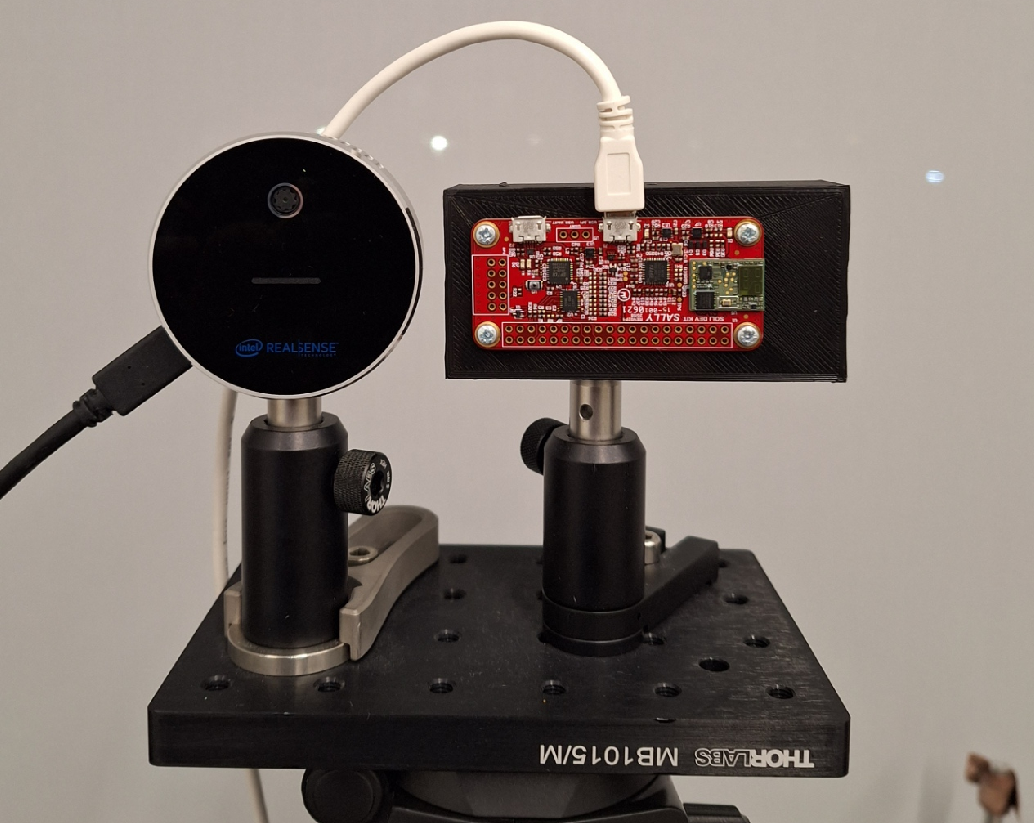
\includegraphics[width=0.35\textwidth,decodearray={1 1 1 1 1 1}]{figures/equipment.pdf}
    \vspace{0.1cm}
    \caption{Equipment: Intel Realsense L515 RGB-D Camera (left) and the Google's Soli \textit{\qty{60}{\GHz}} radar sensor (right)}
    \label{fig:equipment}
    \vspace{-0.3cm}
\end{figure}

\begin{figure}[h!]
    \centering
    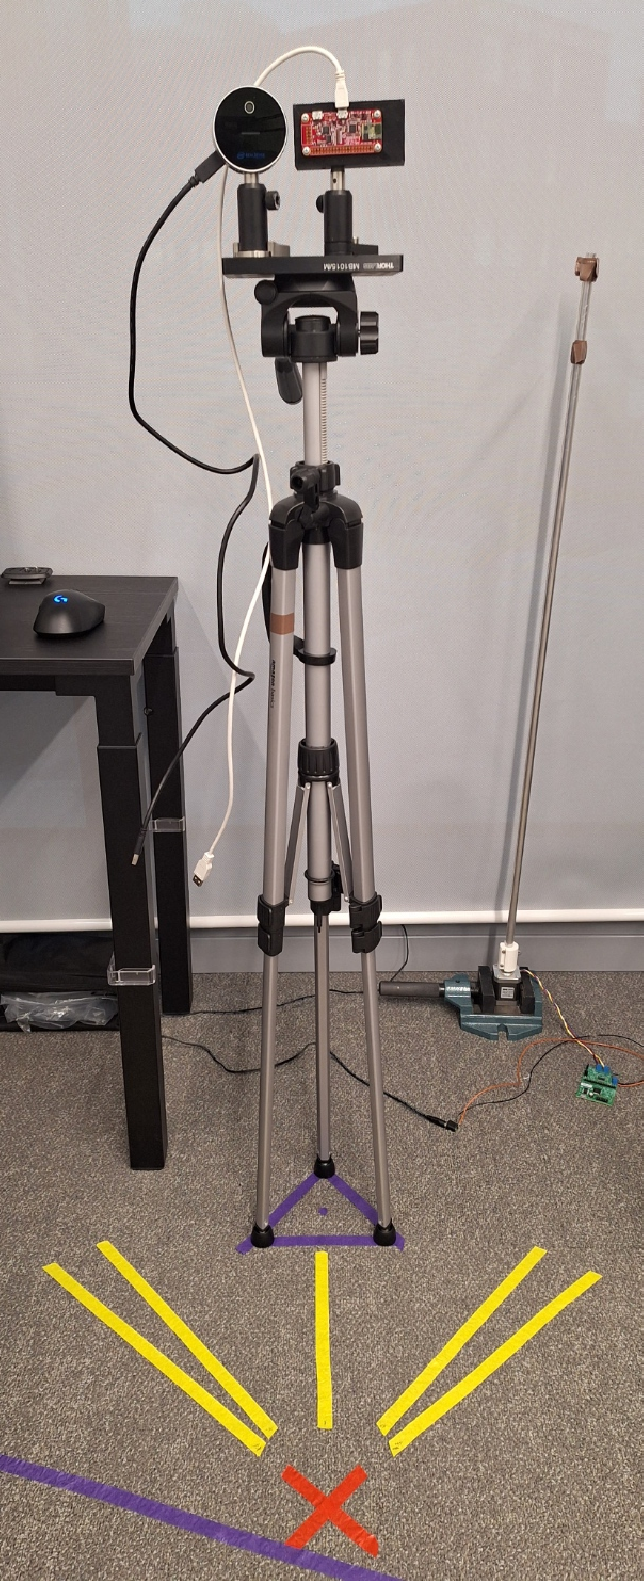
\includegraphics[width=0.31\textwidth, height=12.5cm]{figures/experiment_setup.pdf}
    \vspace{0.2cm}
    \caption{Experiment setup used for data acquisition with the equipment mounted on a tripod. The red cross marks the \qty{20}{\cm} face distance and the yellow tape indicates the five pose directions.}
    \label{fig:experiment_setup}
    \vspace{-0.2cm}
\end{figure}

To illustrate the results of the collection process, the left half of Figure \ref{fig:rgb_crd_plot} presents data samples from a single subject. This grid shows RGB captures from all 15 scenarios, with the three different conditions along the rows and the five pose variations along the columns. For brevity, the experiment conditions are abbreviated as outlined in Table \ref{tab:abbreviated_conditions}.

\begin{table}[h!]
    \centering
    \resizebox{0.4\textwidth}{!}{
        \begin{tabular}{cc}
            \toprule
            \textbf{Abbreviation} & \textbf{Expanded Form} \\
            \midrule
            NO & No Occlusion \\
            O & Occlusion \\
            RLC & Regular Lighting Condition \\
            DLC & Dim Lighting Condition \\
            \bottomrule
        \end{tabular}
    }
    \vspace{0.1cm}
    \caption{Table displaying full forms for abbreviations describing experiment conditions.}
    \label{tab:abbreviated_conditions}
    \vspace{-0.55cm}
\end{table}


% Furthermore, the radar bursts obtained during the data collection phase are preprocessed through multiple FFT stages to transform the raw signals into discretised Complex Range-Doppler (CRD) maps \cite{lien2016soli,hayashi2021radarnet}. This is two-dimensional representation of the reflected radar signal, where the range dimension corresponds to the distance from the Soli sensor and the Doppler dimension corresponds to the radial velocity of the subject towards the sensor. Face scans are collected using the Soli's short configuration which operates at an $f_c$ of \qty{60}{\GHz}, with a maximum bandwidth $B$ of \qty{5.5}{\GHz}, and bursts sampled at \qty{25}{\Hz}. This gives a range resolution of $\frac{c}{2B} = $ \qty{2.7}{\cm}, where $c$ denotes the speed of light. The Soli chip has a single transmit and three receiver antennas, each capturing a superposition of scattered reflections from the target. Given that the Intel RealSense captures RGB-D frames at a different sampling rate of 30 frames per second (FPS), timestamp information is also recorded for the possibility of synchronising the two modalities for early data fusion. The right half of Figure \ref{fig:rgb_crd_plot} illustrates a plot of a single CRD frame across the three receiving channels of the same subject's face. The CRD plot showing the intensities of received signals in discrete 32 Doppler bins along the $x$-axis and 16 Range bins along the $y$-axis.
The radar bursts acquired during the data collection phase undergo multiple FFT stages of preprocessing to convert the raw signals into discretised Complex Range-Doppler (CRD) maps. These maps offer a two-dimensional representation of the reflected radar signal, where the range dimension corresponds to the distance from the Soli sensor, and the Doppler dimension corresponds to the radial velocity of the subject towards the sensor \cite{lien2016soli,hayashi2021radarnet}. Face scans are obtained using the Soli's short configuration, operating at an $f_c$ of \qty{60}{\GHz}, with a maximum bandwidth $B$ of \qty{5.5}{\GHz}. This configuration provides a range resolution $\Delta r$ of:
$$\Delta r = \frac{c}{2B} = \text{\qty{2.7}{\cm}}$$
where $c$ denotes the speed of light. The Soli chip comprises a single transmit and three receiver antennas, each capturing a superposition of scattered reflections from the target. Given that the Intel RealSense captures RGB-D frames at a different sampling rate of 30 frames per second (FPS), timestamp information is also logged for the potential of synchronising the two modalities for early data fusion. The right half of Figure \ref{fig:rgb_crd_plot} depicts a plot of a single CRD frame across the three receiving channels of the same subject's face. The plot illustrates the discrete intensities of received signals across 16 Doppler bins along the $x$-axis and 32 Range bins along the $y$-axis.

\begin{figure*}[h!]
    \centering
    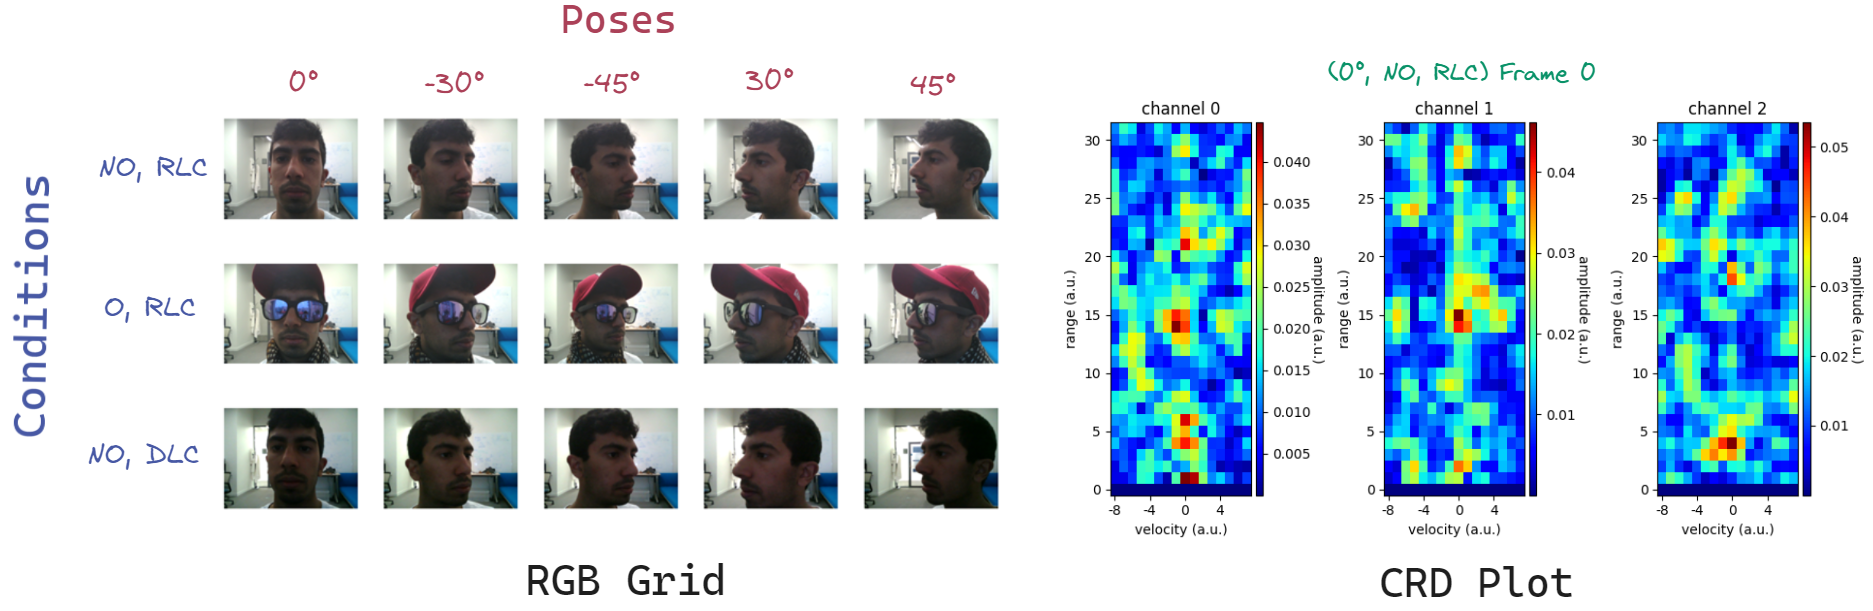
\includegraphics[width=0.99\textwidth]{figures/rgb_crd_plot.png}
    \vspace{0.2cm}
    \caption{Data samples collected for Subject 0. The left figure shows the RGB frames of all 15 scenarios organised by pose and condition. The right figure plots a single CRD frame showing amplitudes of reflected waves detected by the three receiving channels of the Soli, categorised into discrete Range-Doppler bins.}
    \label{fig:rgb_crd_plot}
\end{figure*}


\subsection{mmFace}
Building on the intuition from Section \ref{background:insightface} of the Background chapter, it is clear that the ArcFace model from the InsightFace toolkit emerges as the best choice for our project. It attains state-of-the-art classification results on accepted benchmark sets, outperforming the previous bests such as Facebook's DeepFace \cite{taigman2014deepface} and Google's FaceNet \cite{schroff2015facenet}. This selection allows us to treat the RGB data processing as a \textbf{\textit{black-box}} framework, enabling us to concentrate efforts on perfecting the radar-based feature extraction we are naming, \texttt{mmFace}. Furthermore, this facilitates exploration into the various methods in fusing the two modalities. 

Figure \ref{fig:model_architecture} depicts a high-level diagram of the system workflow employed during training and inference. A more detailed architecture of our end-to-end \texttt{mmFace} model can be viewed in Figure \ref{fig:model_architecture} providing a comprehensive breakdown of each layer as well as their input and output channels. In summary, \texttt{mmFace} takes two inputs: an mmWave face signature in an $\mathtt{ARD}$ format and an InightFace embedding extracted from the corresponding RGB frame. In order to simplify computation, the magnitudes of each complex value, encoding the range $r$ and Doppler $d$ bin, are derived to generate an Absolute Range-Doppler (ARD) map as follows:
$$\mathtt{ARD}_{r,d} = \text{abs}(\mathtt{CRD}_{r,d})$$
The inputs then go through three main stages: \textbf{mmWave Feature Extraction}, \textbf{Feature Fusion}, and \textbf{Class Prediction} each described in detail below to ultimately yield a subject and liveness prediction. The liveness detection is a simple binary classification: 0 denoting a fake subject or 1 for real.
\vspace{-0.1cm}
\begin{enumerate}
    \itemsep0.01cm
    \item \textbf{mmWave Feature Extraction}: Firstly, the $\mathtt{ARD}$ input is processed through four unstrided convolutions followed by a max-pooling then two fully connected layers to compress the radar embedding vector. 
    \item \textbf{Feature Fusion}: The next phase involves fusing the extracted radar embedding with the RGB embedding input. This is modular in design in order to allow any compatible fusion strategy to be employed. This is then processed through a single fully connected layer to reduce its dimensionality before advancing to the final stage. 
    \item \textbf{Class Prediction}: Finally, the fused multimodal embedding is carried across two separate fully connected layers to predict the identity of the face and its authenticity which are subsequently outputted.
\end{enumerate}

\begin{figure*}[h!]
    \centering
    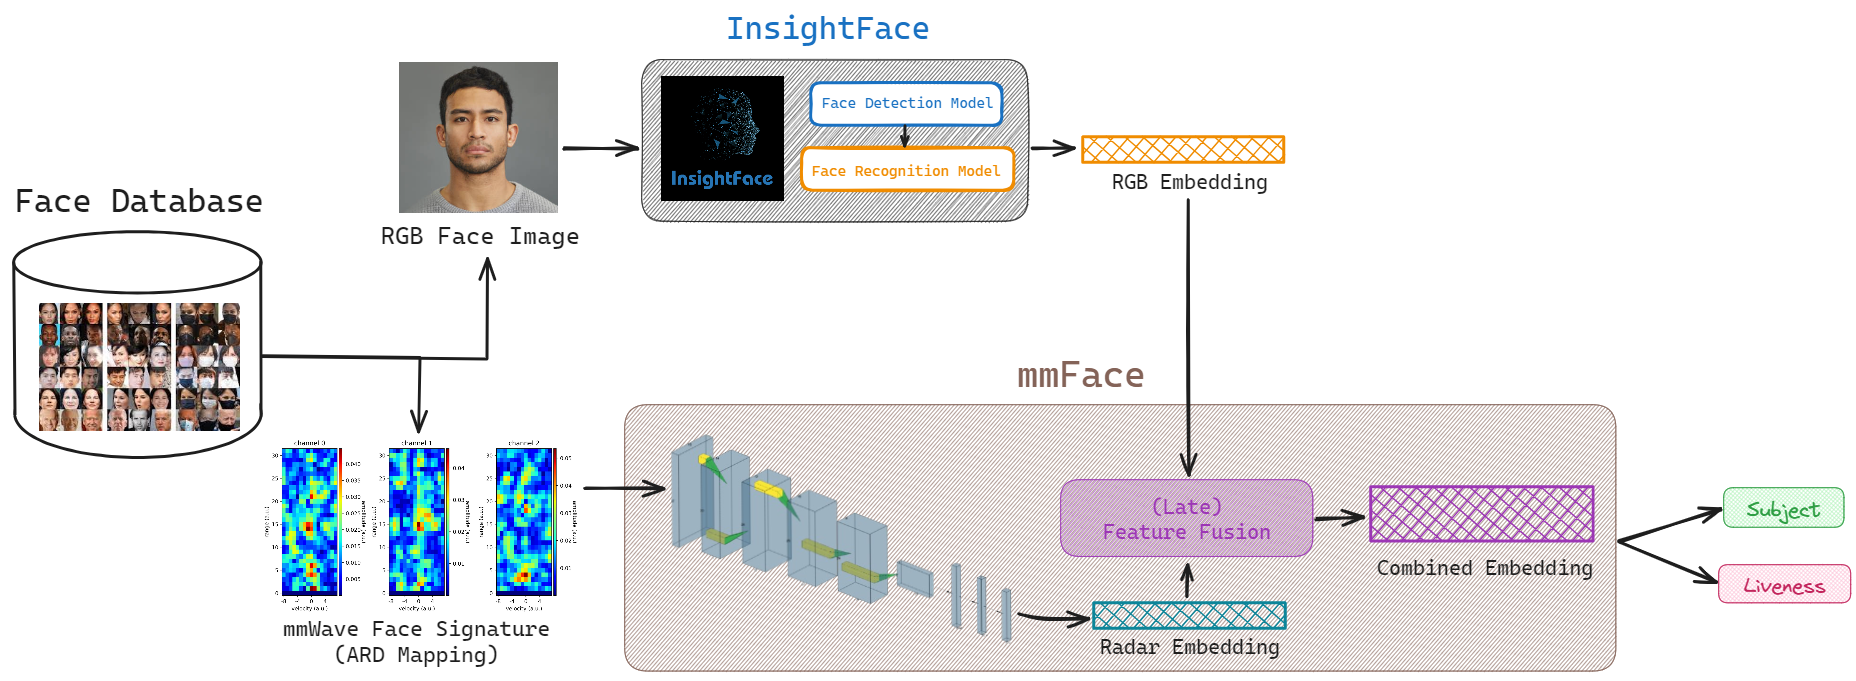
\includegraphics[width=1\textwidth]{figures/model_workflow.png}
    \vspace{0.001cm}
    \caption{High-level model workflow diagram of our proposed 3D face recognition system incorporating millimetre-wave radar and RGB images.}
    \label{fig:model_workflow}
\end{figure*}

\begin{figure*}[h!]
    \centering
    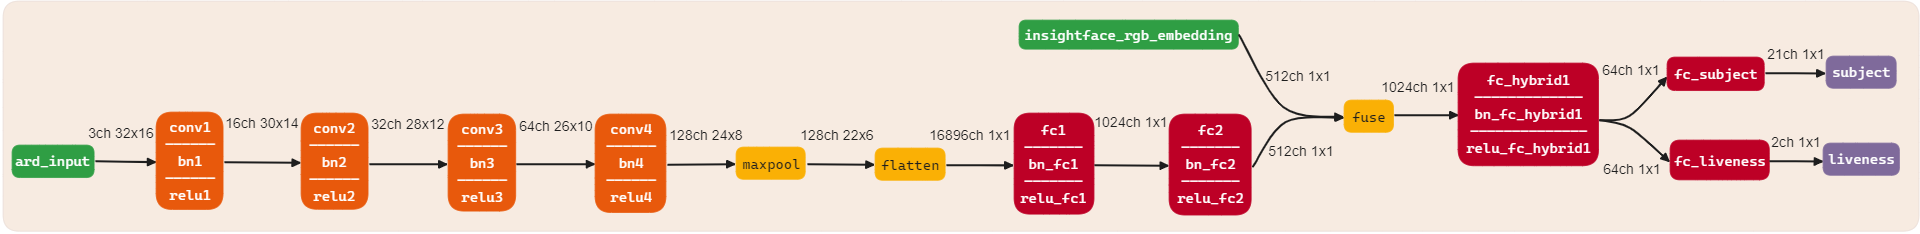
\includegraphics[width=1.02\textwidth]{figures/model_architecture.png}
    \vspace{0.001cm}
    \caption{Model architecture of our \texttt{mmFace} model displaying each layer, as well as its input and output sizes.}
    \label{fig:model_architecture}
\end{figure*}

The three-channel \texttt{ARD} format of the mmWave face signatures allows leveraging convolutional-based feature extraction due to its image-like structure. Convolutional layers would be able to detect spatial patterns among the range and Doppler profiles specific to individual faces, with potential enhancement through deeper layers. Due to the relatively small size of the \texttt{ARD} maps only being $32 \times 16$ bins per channel, it was imperative to preserve most of the information, minimising the need for additional max-poolings or strided convolutions. To streamline the fusion stage, we decided to match the final radar embedding size with the 512-dimension InsightFace feature vector. Four convolution layers with a $3 \times 3$ kernel size and filter sizes sequentially increasing in powers of two starting from 16 to 128 were found to be sufficient, with additional layers affording diminishing returns. All linear transformations are followed by batch normalisation layers to reduce overfitting and increase the generalisability of the model. ReLU activations are chosen for all non-linear transformations to prevent vanishing weights.

We opted to focus on mixing the two modalities within the feature-space, specifically within the network's final layers. This facilitates an easier fusion process since the data from both modalities are abstracted into a compressed representation. Pure intermediate fusion was not feasible due to the black-box treatment of the InsightFace model making it difficult to integrate information from within its hidden layers. Early fusion presents hurdles as well due to the dissimilarities in sampling rates and data formats. The \texttt{ARD} maps have to be synchronised and transformed into a depth image. This is an interesting avenue left to be explored possibly training a neural network to transform the radar bursts into pixel-wise point cloud.

Data augmentations are applied to both \texttt{ARD} and RGB frames, restricted to horizontal and vertical flips due to the distinct nature of both modalities. Augmentations were carefully selected to be semantically consistent across the layout of the mmWave face signatures and colour images. Rotational augmentations, for instance, cannot be seamlessly translated into the range and Doppler bins of the \texttt{ARD} as is the case with traditional images. Data augmentations aimed to introduce positional equivariance and inflate the small dataset size to learn to recognise facial features consistently across different instances.

Ultimately, \texttt{mmFace} contains around 2.8 million parameters and takes, on average, 4.1 milliseconds ($\text{SD}=\text{\qty{0.2}{\ms}}$) to process a single (\texttt{ARD}, RGB-embedding) input pair on an NVIDIA GeForce GTX 1650 GPU.

\subsubsection{Training}
We created and trained our models using PyTorch version 2.1 \cite{paszke2019pytorch}, running for 20 to 25 epochs, employing a Stochastic Gradient Descent (SGD) optimiser that was tasked with minimising the cross entropy losses ($L_{\text{CE}}$) of each prediction. We opted for a fixed learning rate of 0.01, an L2 regularisation rate of $1\mathrm{e}{-3}$, and a momentum of 0.9. As our model generates two predictions, we merge the losses from each with equal weighting to ensure uniform learning of both attributes. This combined loss $\mathcal{L}$ is formulated as follows:
$$\mathcal{L} = L_{\text{CE}}(s, \hat{s}) + L_{\text{CE}}(l, \hat{l})$$
Here, $s$ and $l$ represent the true subject and liveness labels, respectively, while $\hat{s}$ and $\hat{l}$ signify the model's corresponding predictions. 

We train our models on a random subset of 17 out of the total 21 subjects, which accounts for just over an 80\% training split, noting that this includes the 17 fake counterparts, giving 34 total subject instances. The remaining four subjects (or eight instances) are left out for testing.

\subsubsection{Testing}
Our models are evaluated through a zero-shot classification task in order to assess the generalisation ability at identifying unseen faces. During inference, the features from the final hybrid fully connected layer, \texttt{fc\_hybrid1}, are used. The cosine similarity between the final embedding of each test instance and eight pre-selected reference embeddings are calculated to find the maximal score and corresponding prediction for face identity and liveness. A decision threshold $t$ is used such that the maximal score must be greater than it to qualify for a valid prediction. This ensures that predictions are not made for output embeddings that are mostly equidistant to all reference embeddings or too far such that no practical decision can be made.

% Our proposed model, mmFace, will employ a CNN-based architecture, which is particularly effective for processing image-like data. As explained before, the data fusion techniques we plan to investigate include late, feature-level fusion and late, decision-level fusion. Pure intermediate fusion is not feasible due to the black-box treatment of the InsightFace model making it difficult to integrate information from both modalities within its hidden layers. Nonetheless, late, feature-level fusion remains viable, combining the outputs of the final layers of each model to form an embedding containing both the RGB and radar features. Similarly, decision-level fusion will be explored since this entails mixing the predictions from the individual models. Early fusion presents significant challenges due to the dissimilarities in sampling rates and data formats of the two modalities. The CRD maps must be synchronised and transformed into a depth image-like format before merging with the RGB images. Furthermore, this would require a whole new training cycle with the mmFace model which may be infeasible within the project's time frame. However, should time permit, we will consider investigating this approach.

% We plan to adopt a ResNet-based architecture for mmFace due to its refinements over its predecessors like AlexNet \cite{krizhevsky2012imagenet} and VGGNet \cite{simonyan2014very}. The ResNet framework \cite{he2016deep} incorporates ``skip connections'' and residual blocks to resolve the vanishing gradient problem encountered in VGGNet, allowing scaling of the network beyond the 19-layer limitation. This support for deeper networks provides a strong foundation for the mmFace model for learning the complex radar face signatures.

% The dataset, comprising 50 participants, will be divided by subjects into an $80\%/10\%/10\%$ split for training, validation, and testing. Given the dataset's small size, a larger proportion is allocated for training to ensure the model can learn effectively. Following training, the testing phase will evaluate the distinctiveness of the output face embeddings. For accurate classifications, each person's face must be spatially separable in the high-dimensional embedding space allowing for unambiguous identification. t-SNE visualisations \cite{van2008visualizing} will be employed to visually inspect and confirm this is the case by comparing against the original data. In addition, standard classification accuracies will be calculated to verify the model's identity recognition capabilities against randomly selected ground truths. This also allows benchmarking our results against previous studies on radar-based 3D facial recognition.


\subsection{Feature-level Fusion}
% TODO: DIAGRAMS FOR ALL SEVEN FUSIONS?? MULTIHEAD ATTENTION
% TODO: BACKUP WITH SOURCES
We investigate seven feature-level fusion strategies listed as follows in terms of two $n$-dimensional feature vector inputs, $\bm{\vec{x}} = [x_1, x_2, \ldots, x_n]$ and $\bm{\vec{y}} = [y_1, y_2, \ldots, y_n]$:
\vspace{-0.1cm}
\begin{enumerate}
    \itemsep0em
    \item \textbf{Concatenate:} This is a straightforward concatenation of the two feature vectors, the most common strategy employed for its ease of implementation and effectiveness as all information is preserved.
    $$\mathtt{concatenate}(\bm{\vec{x}}, \bm{\vec{y}}) = [\bm{\vec{x}}, \bm{\vec{y}}]$$

    \item \textbf{Add:} This involves an element-wise vector addition of $\bm{\vec{x}}$ and $\bm{\vec{y}}$. This can be highly effective when both feature vectors point in the same direction compounding their resulting summation, however, if both feature vectors point in opposite directions, then this would result in a more orthogonal resulting vector direction.
    % $$\mathtt{add}(\bm{\vec{x}}, \bm{\vec{y}}) = [x_1 + y_1, x_2 + y_2, \ldots, x_n + y_n]$$
    $$\mathtt{add}(\bm{\vec{x}}, \bm{\vec{y}}) = \left[(x_i + y_i) \ | \ \forall i \in \{1, \ldots, n\}\right]$$
    
    \item \textbf{Hadamard Product:} This is the element-wise vector multiplication or the Hadamard product of $\bm{\vec{x}}$ and $\bm{\vec{y}}$. The idea here is to preserve the original feature vector structure while emphasising relationships between corresponding feature elements. It has been used successfully for multimodal residual learning by Kim et al. \cite{kim2016multimodal}.
    % $$\mathtt{hadamard\_product}(\bm{\vec{x}}, \bm{\vec{y}}) = [x_1 \cdot y_1, x_2 \cdot y_2, \ldots, x_n \cdot y_n]$$
    $$\mathtt{hadamard\_product}(\bm{\vec{x}}, \bm{\vec{y}}) = \left[(x_iy_i) \ | \ \forall i \in \{1, \ldots, n\}\right]$$
    
    \item \textbf{Pairwise Dot Mean:} This involves a dot product of the transpose of vector $\bm{\vec{x}}$ with vector $\bm{\vec{y}}$ resulting in an $n \times n$ matrix followed by a column-wise mean operation to produce an $n$-dimensional fused feature vector. The rationale behind this stems from the pairwise dot providing a more comprehensive blending of the feature. Each radar feature is multiplied by every RGB feature, and the resulting values are all attended to during the pooling process to reduce the dimensionality of the matrix.
    \begin{align*}
        \mathit{Let} \ \bm{Z} & = \ \bm{\vec{x}}^T \cdot \bm{\vec{y}} \ \mathit{in} \\
        % \mathtt{pairwise\_dot\_average}&(\bm{\vec{x}}, \bm{\vec{y}}) =\\& \left[ \frac{1}{n} \sum_{i=1}^n \bm{Z}_{i,1}, \frac{1}{n} \sum_{i=1}^n \bm{Z}_{i,2}, \ldots, \frac{1}{n} \sum_{i=1}^n \bm{Z}_{i,n} \right] \\
        \hspace{-0.2cm}\mathtt{pairwise\_dot\_mean}(\bm{\vec{x}}, \bm{\vec{y}}) &= \left[ \frac{1}{n} \sum_{j=1}^n \bm{Z}_{j,i} \ \middle| \ \forall i \in \{1, \ldots, n\}\right]
    \end{align*}
    
    \item \textbf{Pairwise Dot Max:} This similarly involves the dot product followed by a column-wise max. In contrast to averaging, which could squash certain feature correlations, this approach isolates larger features resulting from the exhaustive mixing of both modalities, a similar intuition behind the max-pooling layers. Here, $*$ denotes a selection of all rows of a matrix.
    \begin{align*}
        \mathit{Let} \ \bm{Z} & = \bm{\vec{x}}^T \cdot \bm{\vec{y}} \ \mathit{in} \\
        % \mathtt{pairwise\_dot\_max}(\bm{\vec{x}}, &\bm{\vec{y}}) =\\ &\left[ \max(\bm{Z}_{*,1}), \max(\bm{Z}_{*,2}), \ldots, \max(\bm{Z}_{*,n}) \right] \\
        \mathtt{pairwise\_dot\_max}(\bm{\vec{x}}, \bm{\vec{y}}) &= \left[ \max(\bm{Z}_{*,i}) \ \middle| \ \forall i \in \{1, \ldots, n\} \right]
    \end{align*}
    
    \item \textbf{Pairwise Dot Flatten:} This is the final pairwise dot fusion strategy now following the dot product with a flatten operation of the $n \times n$ matrix into an $n^2$-dimensional vector. This conversely retains all correlations between the radar and RGB features, leaving the subsequent fully connected layers of the model to determine which features are most relevant.
    \begin{align*}
        \mathit{Let} \ \bm{Z} = & \ \bm{\vec{x}}^T \cdot \bm{\vec{y}} \ \mathit{in} \\
        \mathtt{pairwise\_dot\_flatten}(\bm{\vec{x}}, &\bm{\vec{y}}) =\\ &\left[ \bm{Z}_{1,1}, \bm{Z}_{1,2}, \ldots, \bm{Z}_{n,n\text{-}1}, \bm{Z}_{n,n} \right]
    \end{align*}
    
    \item \textbf{Multi-Head Attention:} This involves using a self-attention mechanism prevalent in transformer architectures popularised by the seminal paper by Vaswani et al. \cite{vaswani2017attention}. It was initially designed for natural language processing tasks but has shown a lot of success in computer vision. The key idea of self-attention is to isolate and mix the most important aspects from both feature vectors by converting them into three distinct representations: a query $\bm{Q}$, key $\bm{K}$, and value $\bm{V}$. Each embedding plays a unique role such as the query capturing features that the model deems relevant for making predictions. To do this $\bm{Q}$ may focus on features that are shared or discriminative across both modalities such as facial landmarks and overall identity information. Meanwhile, $\bm{K}$ might focus on modality-specific elements such as the colour and texture information embedded within the RGB feature vector, while 3D structural details being offered by the radar embedding. Finally, $\bm{V}$ encapsulates the actual fine-grained details captured by both modalities that will be attended to by the model based on the resulting query-key similarities. In order to maximise this affect, this mechanism is applied separately across multiple attention heads, reducing the risk of overlooking salient characteristics.
    This is expressed formally below, where first the two inputs are stacked vertically, $\bm{X} = \begin{bmatrix} \bm{\vec{x}} \\ \bm{\vec{y}} \end{bmatrix}$, then copied through three separate linear transformations to obtain the $\bm{Q}$, $\bm{K}$, $\bm{V}$ matrices. This is done for each of the $k$ attention heads using separate learnable weight matrices.
    % TODO: HOW ATTENTION FROM PYTORCH DOCS
    % TODO: POSITIONAL ENCODING??
    \begin{align*}
        \mathit{Let} \ h_i = \mathtt{Attention}(\bm{Q}_i&, \bm{K}_i, \bm{V}_i) \ \mathit{in} \\
        \hspace{-1cm}\mathtt{multihead\_attention}(\bm{\vec{x}}, \bm{\vec{y}}) &= [h_1, \ldots, h_k]\bm{W}^O \\
        \mathit{where} \ 
        % \bm{X} = 
        % \begin{bmatrix}
        %     \bm{\vec{x}} \\
        %     \bm{\vec{y}}
        % \end{bmatrix} 
        % \bm{Q}_i = \bm{W}_{Q_i}\bm{X}, \ \bm{K}_i = \bm{W}_{K_i}&\bm{X} \ \mathit{and} \ \bm{V}_i = \bm{W}_{V_i}\bm{X}
        \bm{Q}_i = \bm{W}^{Q}_i\bm{X}, \ \bm{K}_i = \bm{W}^{K}_i&\bm{X} \ \mathit{and} \ \bm{V}_i = \bm{W}^{V}_i\bm{X}
    \end{align*}
\end{enumerate}



\section{Evaluation}
We evaluate our model by examining its discriminative ability at representing the four unseen faces. We utilise various metrics, such as the prediction accuracies, precision and recall, and ROC AUC, to compare the different fusion strategies against each other as well showing their performance against simply using the individual modalities. Prior to the zero-shot task, we select and extract the final hidden representation of eight reference frame pairs. These reference embeddings serve as the basis for comparison with the test set, encompassing both live and fake samples of the four unseen subjects.

\subsection{Results}
Firstly, we gauge the accuracies of the models in predicting both the facial identity and authenticity. This involves determining the most similar reference embedding to the final feature vector of a specific test sample using the maximum cosine similarity. A decision threshold $t$ of 0.5 is applied to quantify a true prediction, otherwise, it is marked as a failed prediction. All models demonstrate high coverage, as illustrated in Table \ref{tab:averaged_acc_fb}, with the radar-only model achieving the lowest coverage at 79.8\%. Secondly, since the eight selected reference instances exhibit two properties -- facial identity and liveness status -- this allows for the calculation of separate metrics to assess each model's ability to predict identity independently of the liveness check.

\subsubsection{Accuracy and F-measure}
Table \ref{tab:subject_liveness_acc_fb} presents the subject and liveness accuracies for all feature fusion strategies as well as the weighted $F_{\beta}$-measures, averaged over all the respective classes. For completeness, the performance of the individual modalities are also listed in order to show the advantageous effect of the multimodal feature fusions. A $\beta$ value of 0.5 was chosen for the F-scores since, in face recognition systems, erroneously admitting the wrong identity is more detrimental than false negatives, thus requiring twice the emphasis on precision compared to recall.

\begin{table}[htbp]
    \centering
    \resizebox{1.02\columnwidth}{1.9cm}{
        \begin{tabular}{lcccc}
            \toprule
            \multirow{2}{*}{\textbf{Fusion Strategy}} & \multicolumn{2}{c}{\textbf  {Subject}} & \multicolumn{2}{c}{\textbf{Liveness}} \\
            \cmidrule(lr){2-3} \cmidrule(lr){4-5} & \textbf{Accuracy (\%)} & \textbf{$\bm{F_{0.5}}$ Score} & \textbf{Accuracy (\%)} & \textbf{$\bm{F_{0.5}}$ Score} \\
            \midrule
            Concatenate & 83.7 & 0.835 & \cellcolor{lightgreen}99.6 & \cellcolor{lightgreen}0.996 \\
            Add & \cellcolor{lightred}63.0 & \cellcolor{lightred}0.629 & 99.2 & 0.992 \\
            Hadamard Product & 87.1 & 0.869 & 96.7 & 0.963 \\
            Pairwise Dot Mean & \cellcolor{lightgreen}88.8 & \cellcolor{lightgreen}0.880 & 80.8 & 0.808 \\
            Pairwise Dot Max & 82.7 & 0.820 & \cellcolor{lightred}72.8 & \cellcolor{lightred}0.735 \\
            Pairwise Dot Flatten & 86.7 & 0.862 & 94.7 & 0.944 \\
            Multi-Head Attention & 86.3 & 0.851 & 96.4 & 0.950 \\
            \midrule
            Radar Only & 38.2 & 0.370 & 96.6 & 0.916 \\
            RGB Only & 85.5 & 0.855 & 69.3 & 0.701 \\
            \bottomrule
        \end{tabular}
    }
    \vspace{0.1cm}
    \caption{Subject and liveness accuracies and weighted-averaged $F_{0.5}$ measures for the seven feature fusion strategies along with the individual modalities.}
    \label{tab:subject_liveness_acc_fb}
    \vspace{-0.1cm}
\end{table}

% TODO: Discuss results of individual modalities
The best and worst performers are highlighted in green and red respectively. Evidently, certain fusion strategies excel at identifying subjects, while others are more adept at predicting face liveness. Among these strategies, the concatenation method emerges as the most effective for accurately verifying liveness. Meanwhile, the pairwise dot then mean strategy outperforms within the subject category, attaining the highest accuracy and $F_{0.5}$ measure. However, it's ability to detect face liveness is notably lacking, obtaining an accuracy that is even lower than simply using the mmWave radar features. This is likely due to the mean pooling step squashing outlier feature correlations between the two modalities that may be relevant for the liveness detection. The vector addition proves to be very ineffective in predicting facial identity, being much better at predicting liveness in comparison. 

Examining the individual performance for each prediction type provides insight into the strategies' effectiveness in classifying unseen data to their respective labels. However, it's equally important to identify the overall best strategy that performs well in both categories.

Table \ref{tab:averaged_acc_fb} showcases each of the nine models with their respective average accuracy and $F_{0.5}$ measure applying equal weighting to the subject and liveness results. It is evident that the Hadamard product of the two feature vectors achieved the highest mean accuracy and F-measure. Additionally, it highlights the fact that all fusion strategies improve on the results from using the independent modalities alone.

\begin{table}[htbp]
    \centering
    \resizebox{1.01\columnwidth}{1.7cm}{
        % \begin{tabular}{lS[table-format=2.2]S[table-format=1.4]}
        \begin{tabular}{lccc}
            \toprule
            \textbf{Fusion Strategy}   & {\textbf{Mean Accuracy (\%)}} & {\textbf{Mean $\bm{F_{0.5}}$ Score}} & \textbf{Coverage (\%)} \\
            \midrule
            Concatenate          & 91.7 & 0.915 & 99.7 \\
            Add                  & 81.1 & 0.811 & 99.9 \\
            \rowcolor{lightgreen}
            Hadamard Product  & 91.9 & 0.916 & 98.1 \\
            Pairwise Dot Mean    & 84.8 & 0.844 & 95.3 \\
            \rowcolor{lightred}
            Pairwise Dot Max     & 77.8 & 0.778 & 95.6 \\
            Pairwise Dot Flatten & 90.7 & 0.903 & 97.8 \\
            Multi-Head Attention & 91.3 & 0.900 & 92.5 \\
            \midrule
            Radar Only           & 67.4 & 0.643 & 79.8 \\
            RGB Only             & 77.4 & 0.778 & 97.5 \\
            \bottomrule
        \end{tabular}
    }
    \vspace{0.1cm}
    \caption{Averaged accuracy and $F_{0.5}$ score for the seven fusion strategies and individual modalities, applying equal weighting to subject and liveness predictions.}
    \label{tab:averaged_acc_fb}
    \vspace{-0.3cm}
\end{table}

\subsubsection{ROC Curves and AUC}
However, it is notable that the element-wise product method is closely followed by the concatenation and multi-head attention strategies therefore it is more informative to assess the model's performance at different decision thresholds. This is the main idea behind the Receiver Operating Characteristic (ROC) Curve which analyses the true positive rate (TPR) against the false positive rate (FPR) at varying decision thresholds. However, given the multi-classification nature of our task, the one-vs-the-rest (OvR) ROC curve is more appropriate, where each class is evaluated against the rest using a one-hot strategy. This therefore, needs each of the eight reference test subjects to be plotted separately.

Figure \ref{fig:roc_hadamard_product} plots the one-vs-the-rest ROC curves for the highest performing strategy: feature fusion by the Hadamard product. The blue dotted curve indicates the macro-averaged trend among the individual curves, while the dashed diagonal line denotes the chance level equivalent to a random guessing model. Curves above the chance level and reaching the top-left corner demonstrate a better classifier. This is often quantified by the area under the curve (AUC) metric of the ROC curve. 

\begin{figure*}[h!]
    \centering
    \begin{subfigure}[b]{0.31\textwidth}
        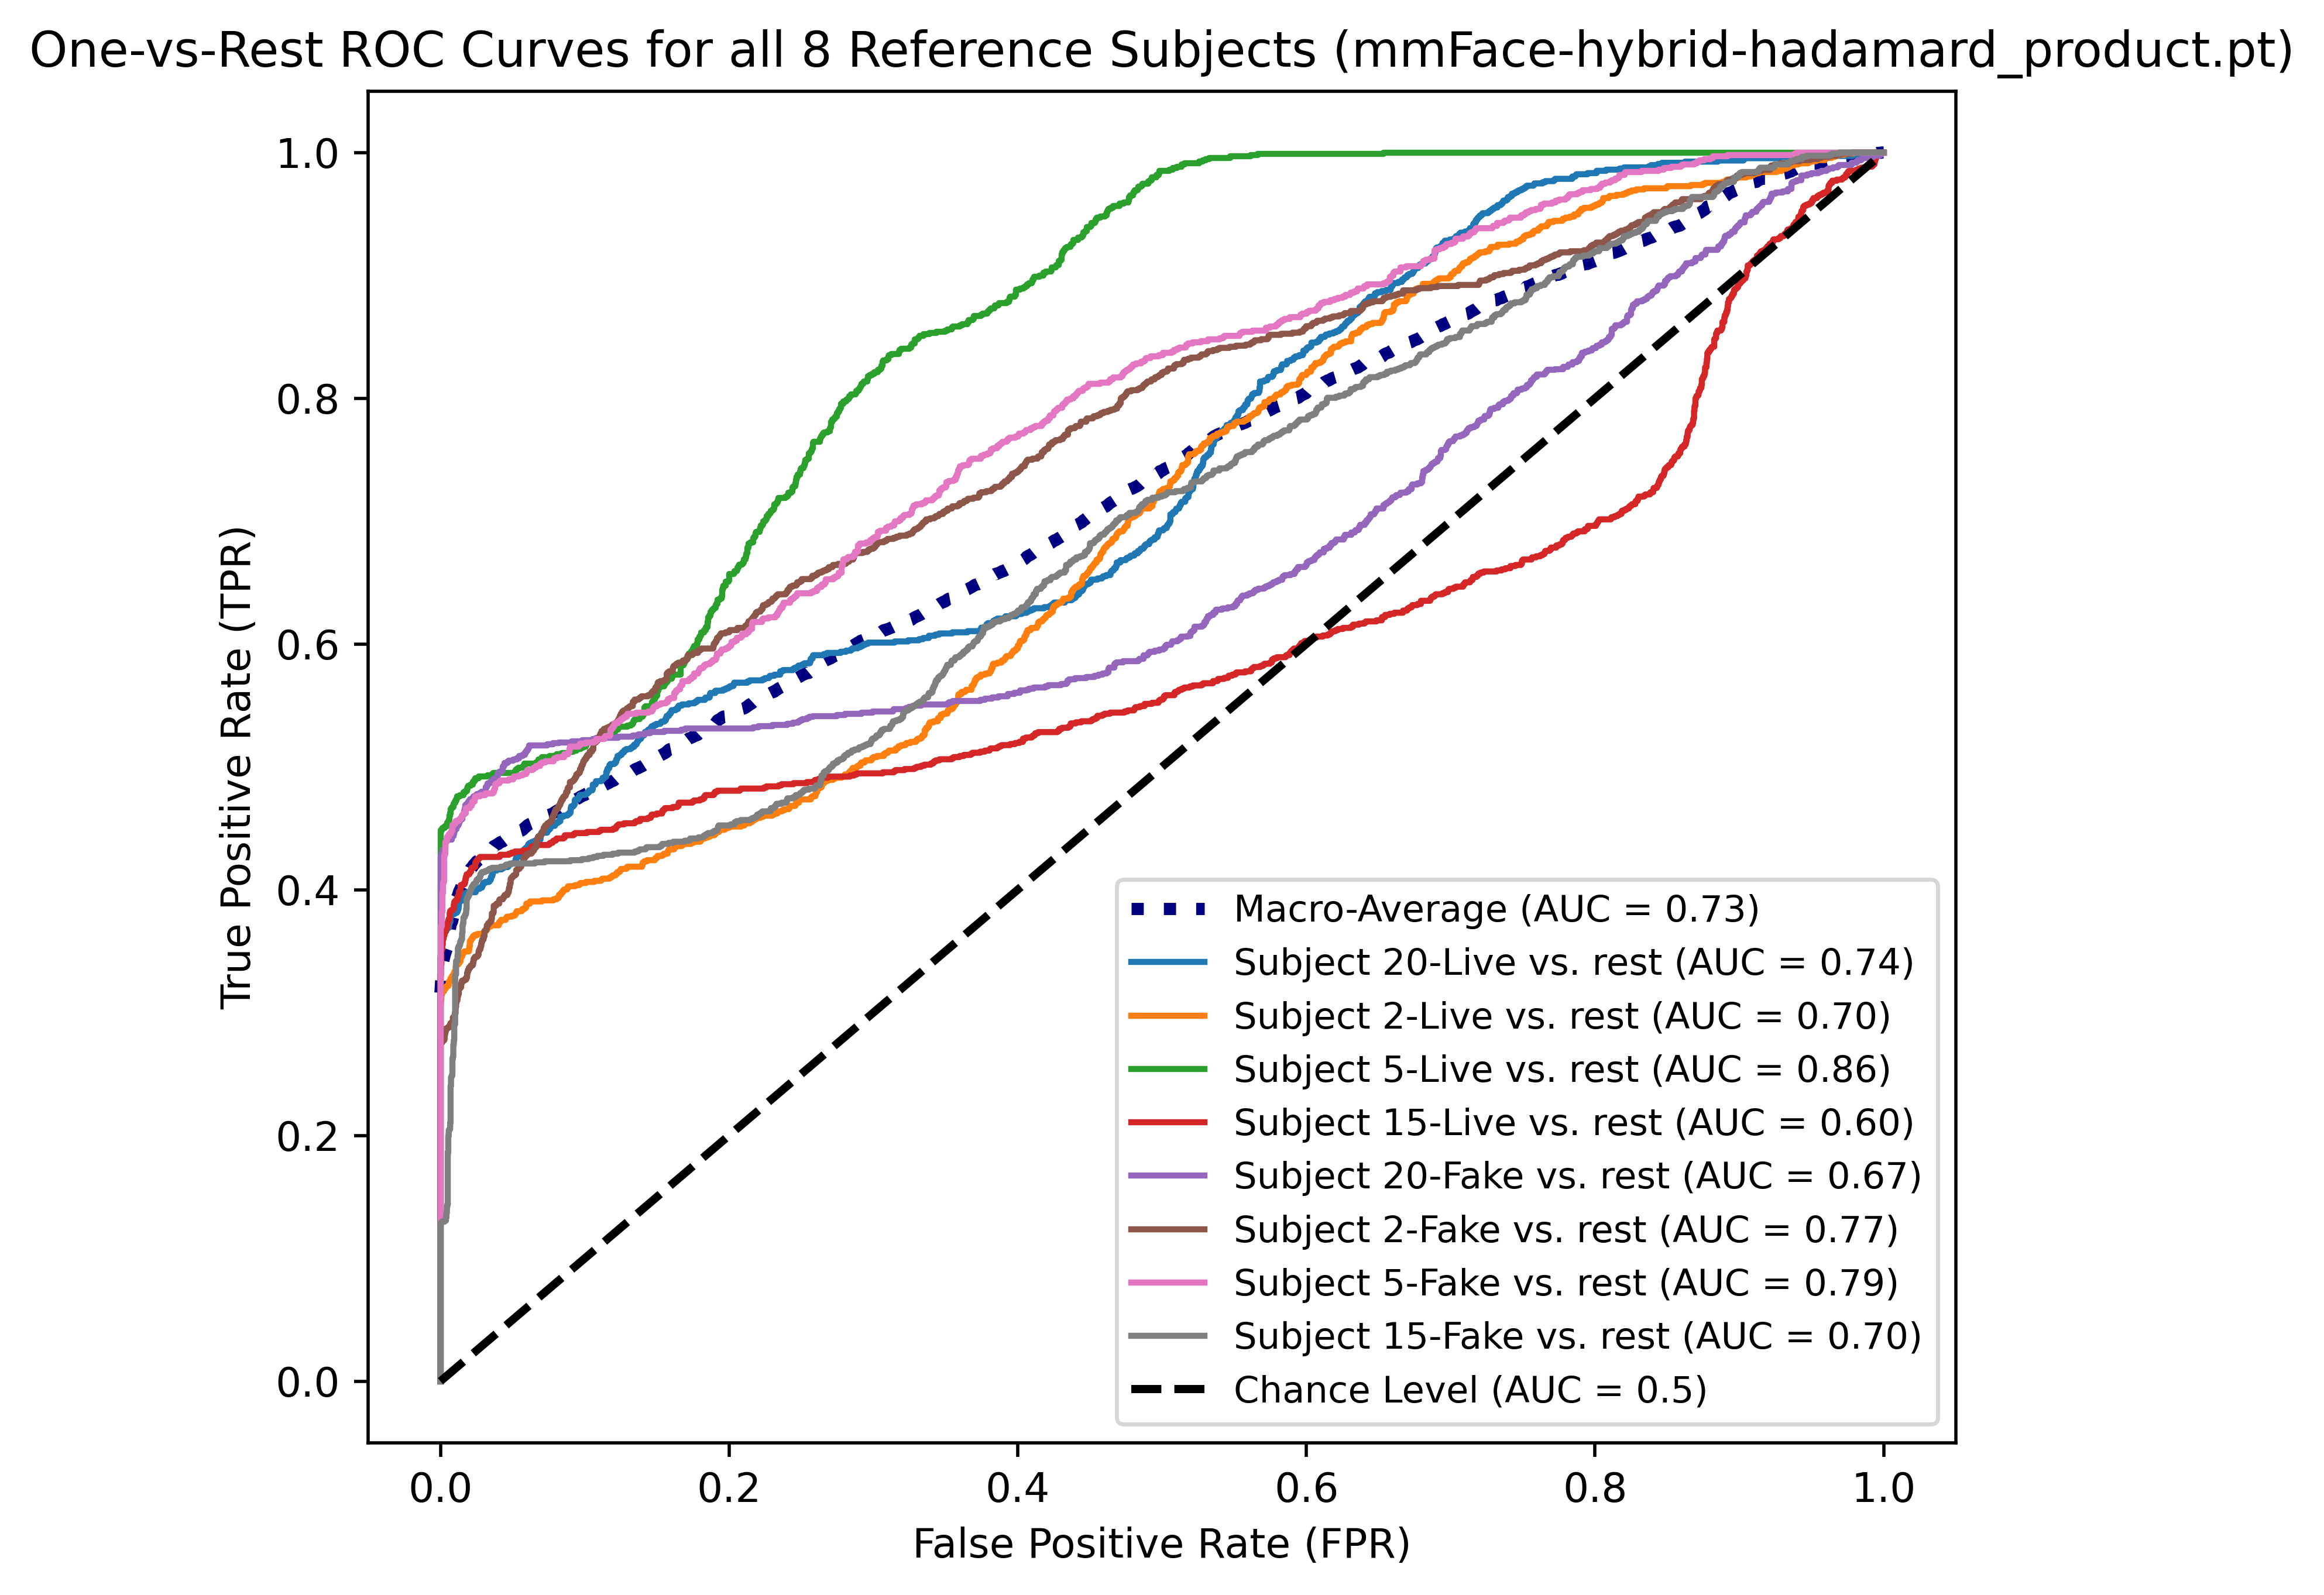
\includegraphics[width=\textwidth]{figures/roc_hadamard_product.png}
        \caption{Hadamard Product}
        \label{fig:roc_hadamard_product}
    \end{subfigure}
    ~
    \begin{subfigure}[b]{0.3\textwidth}
        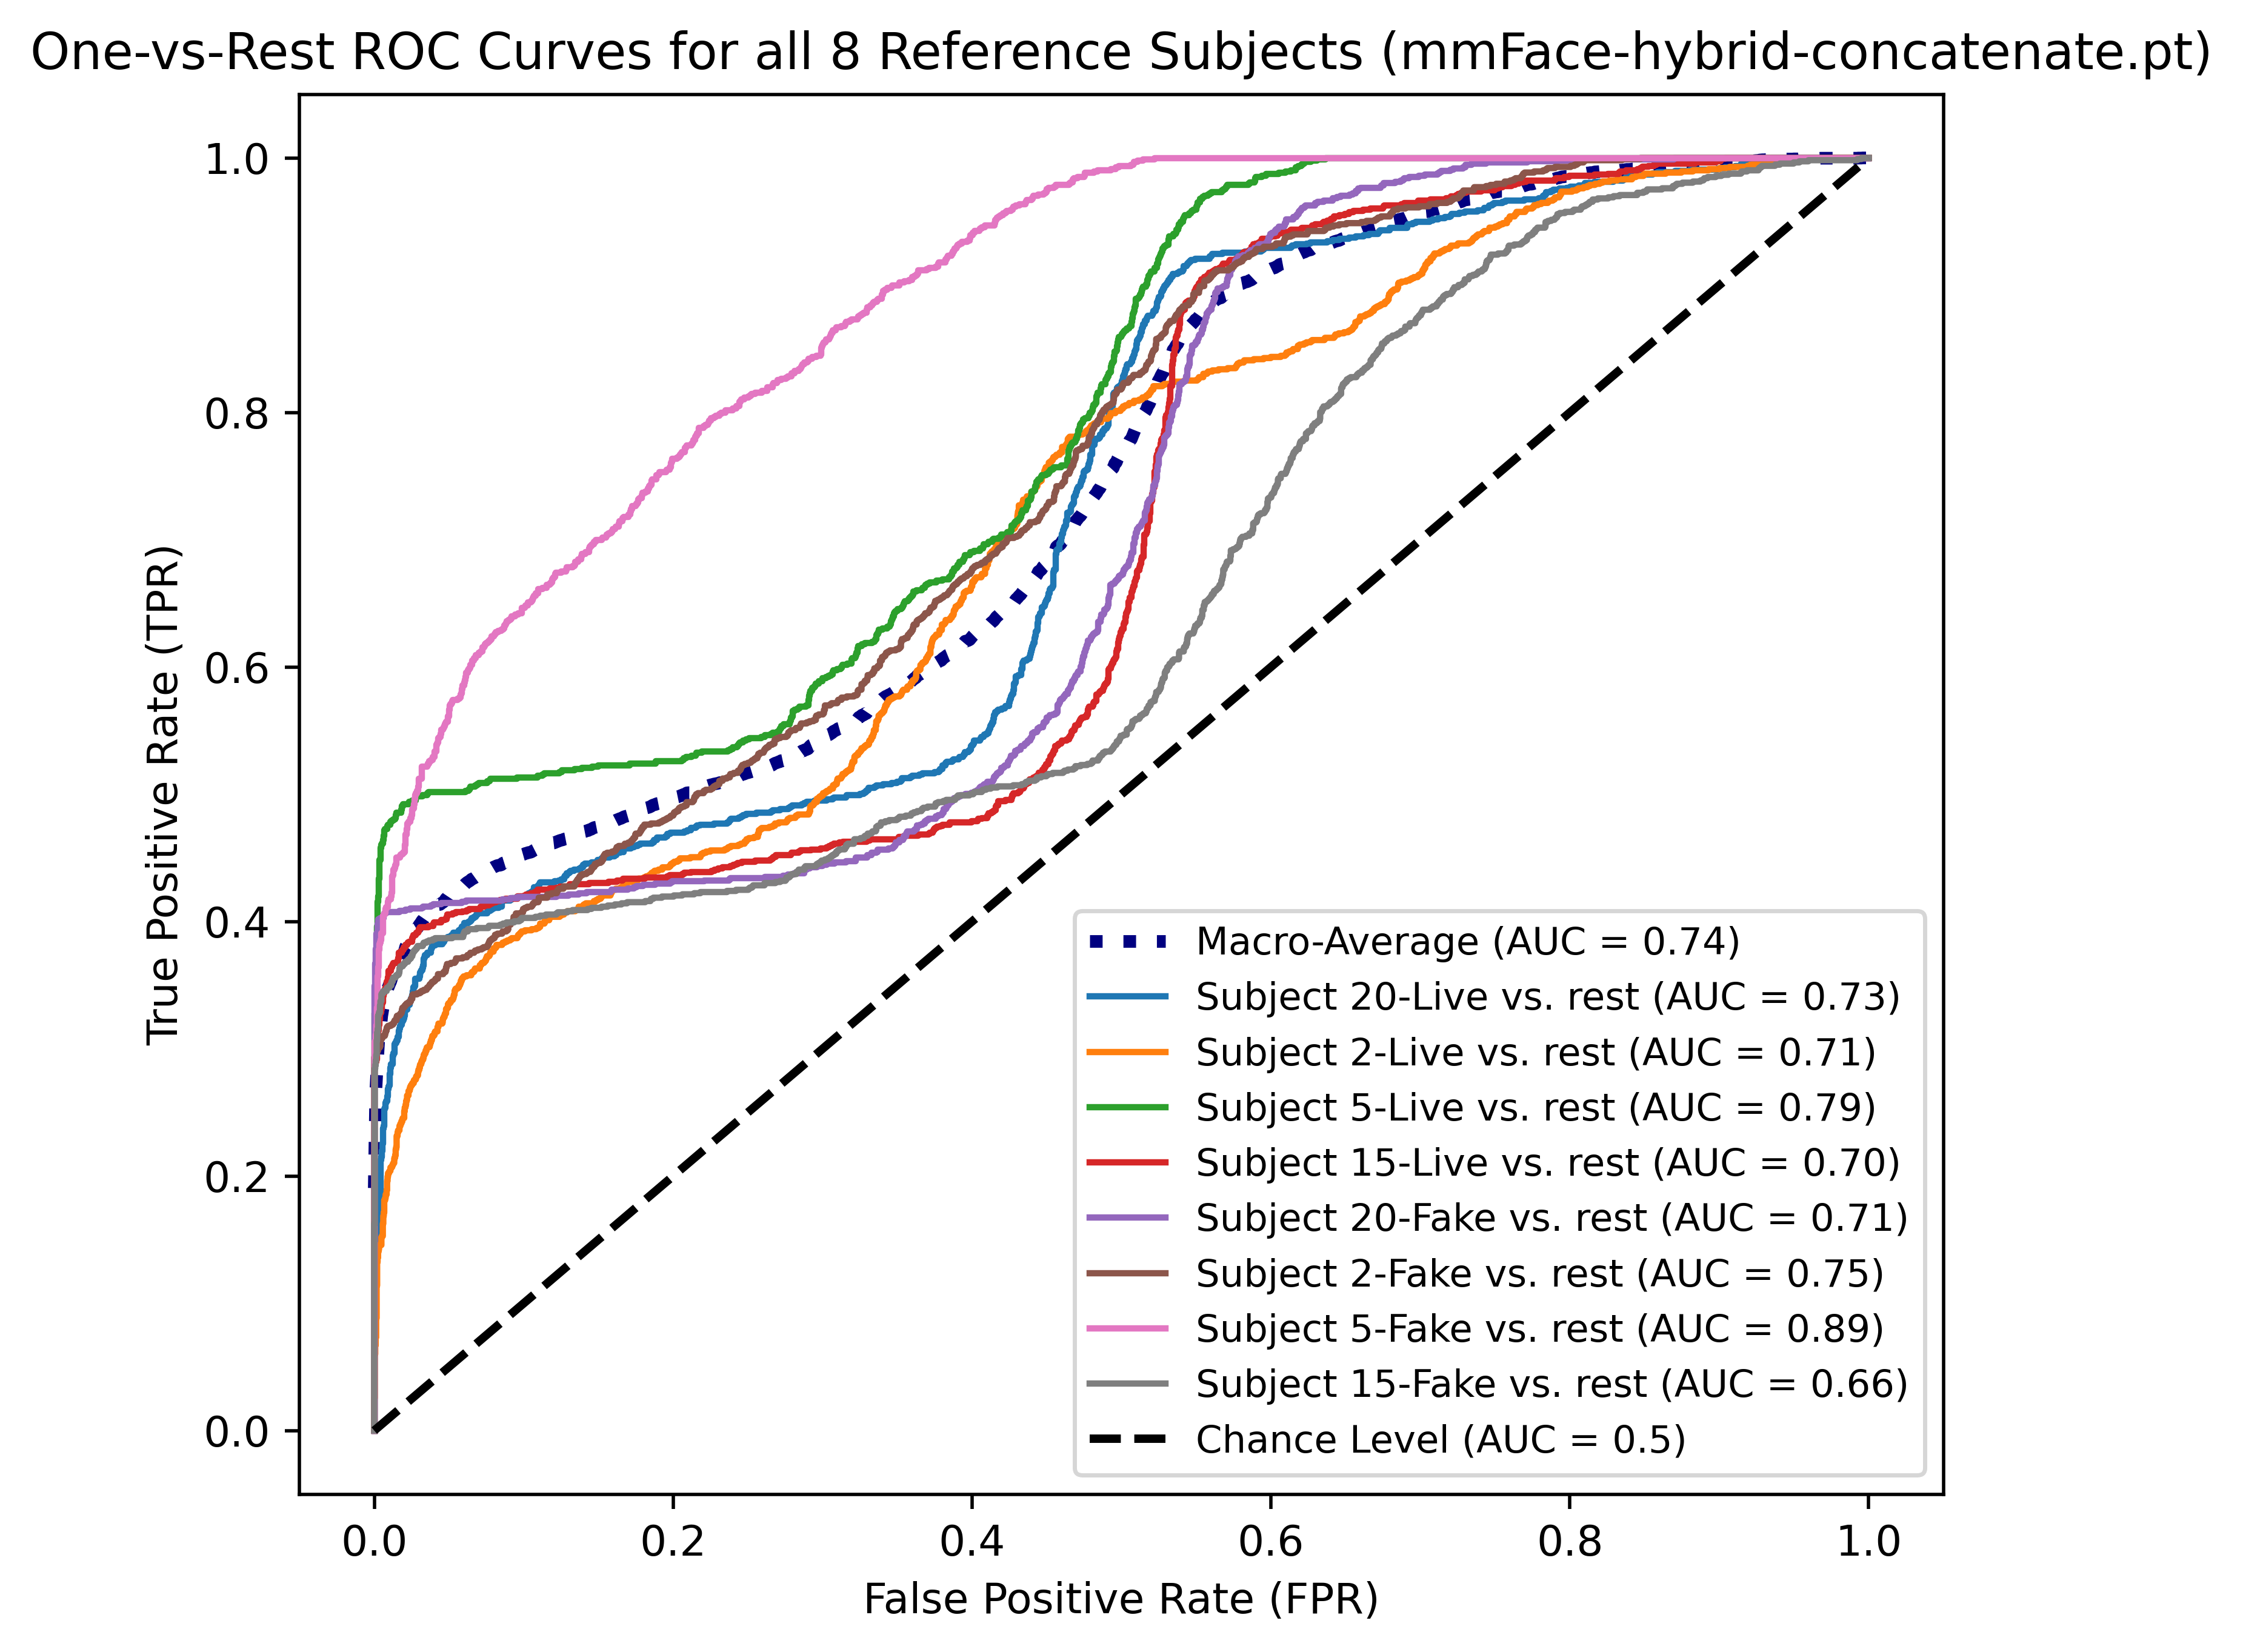
\includegraphics[width=\textwidth]{figures/roc_concatenate.png}
        \caption{Concatenate}
        \label{fig:roc_concatenate}
    \end{subfigure}
    ~
    \begin{subfigure}[b]{0.31\textwidth}
        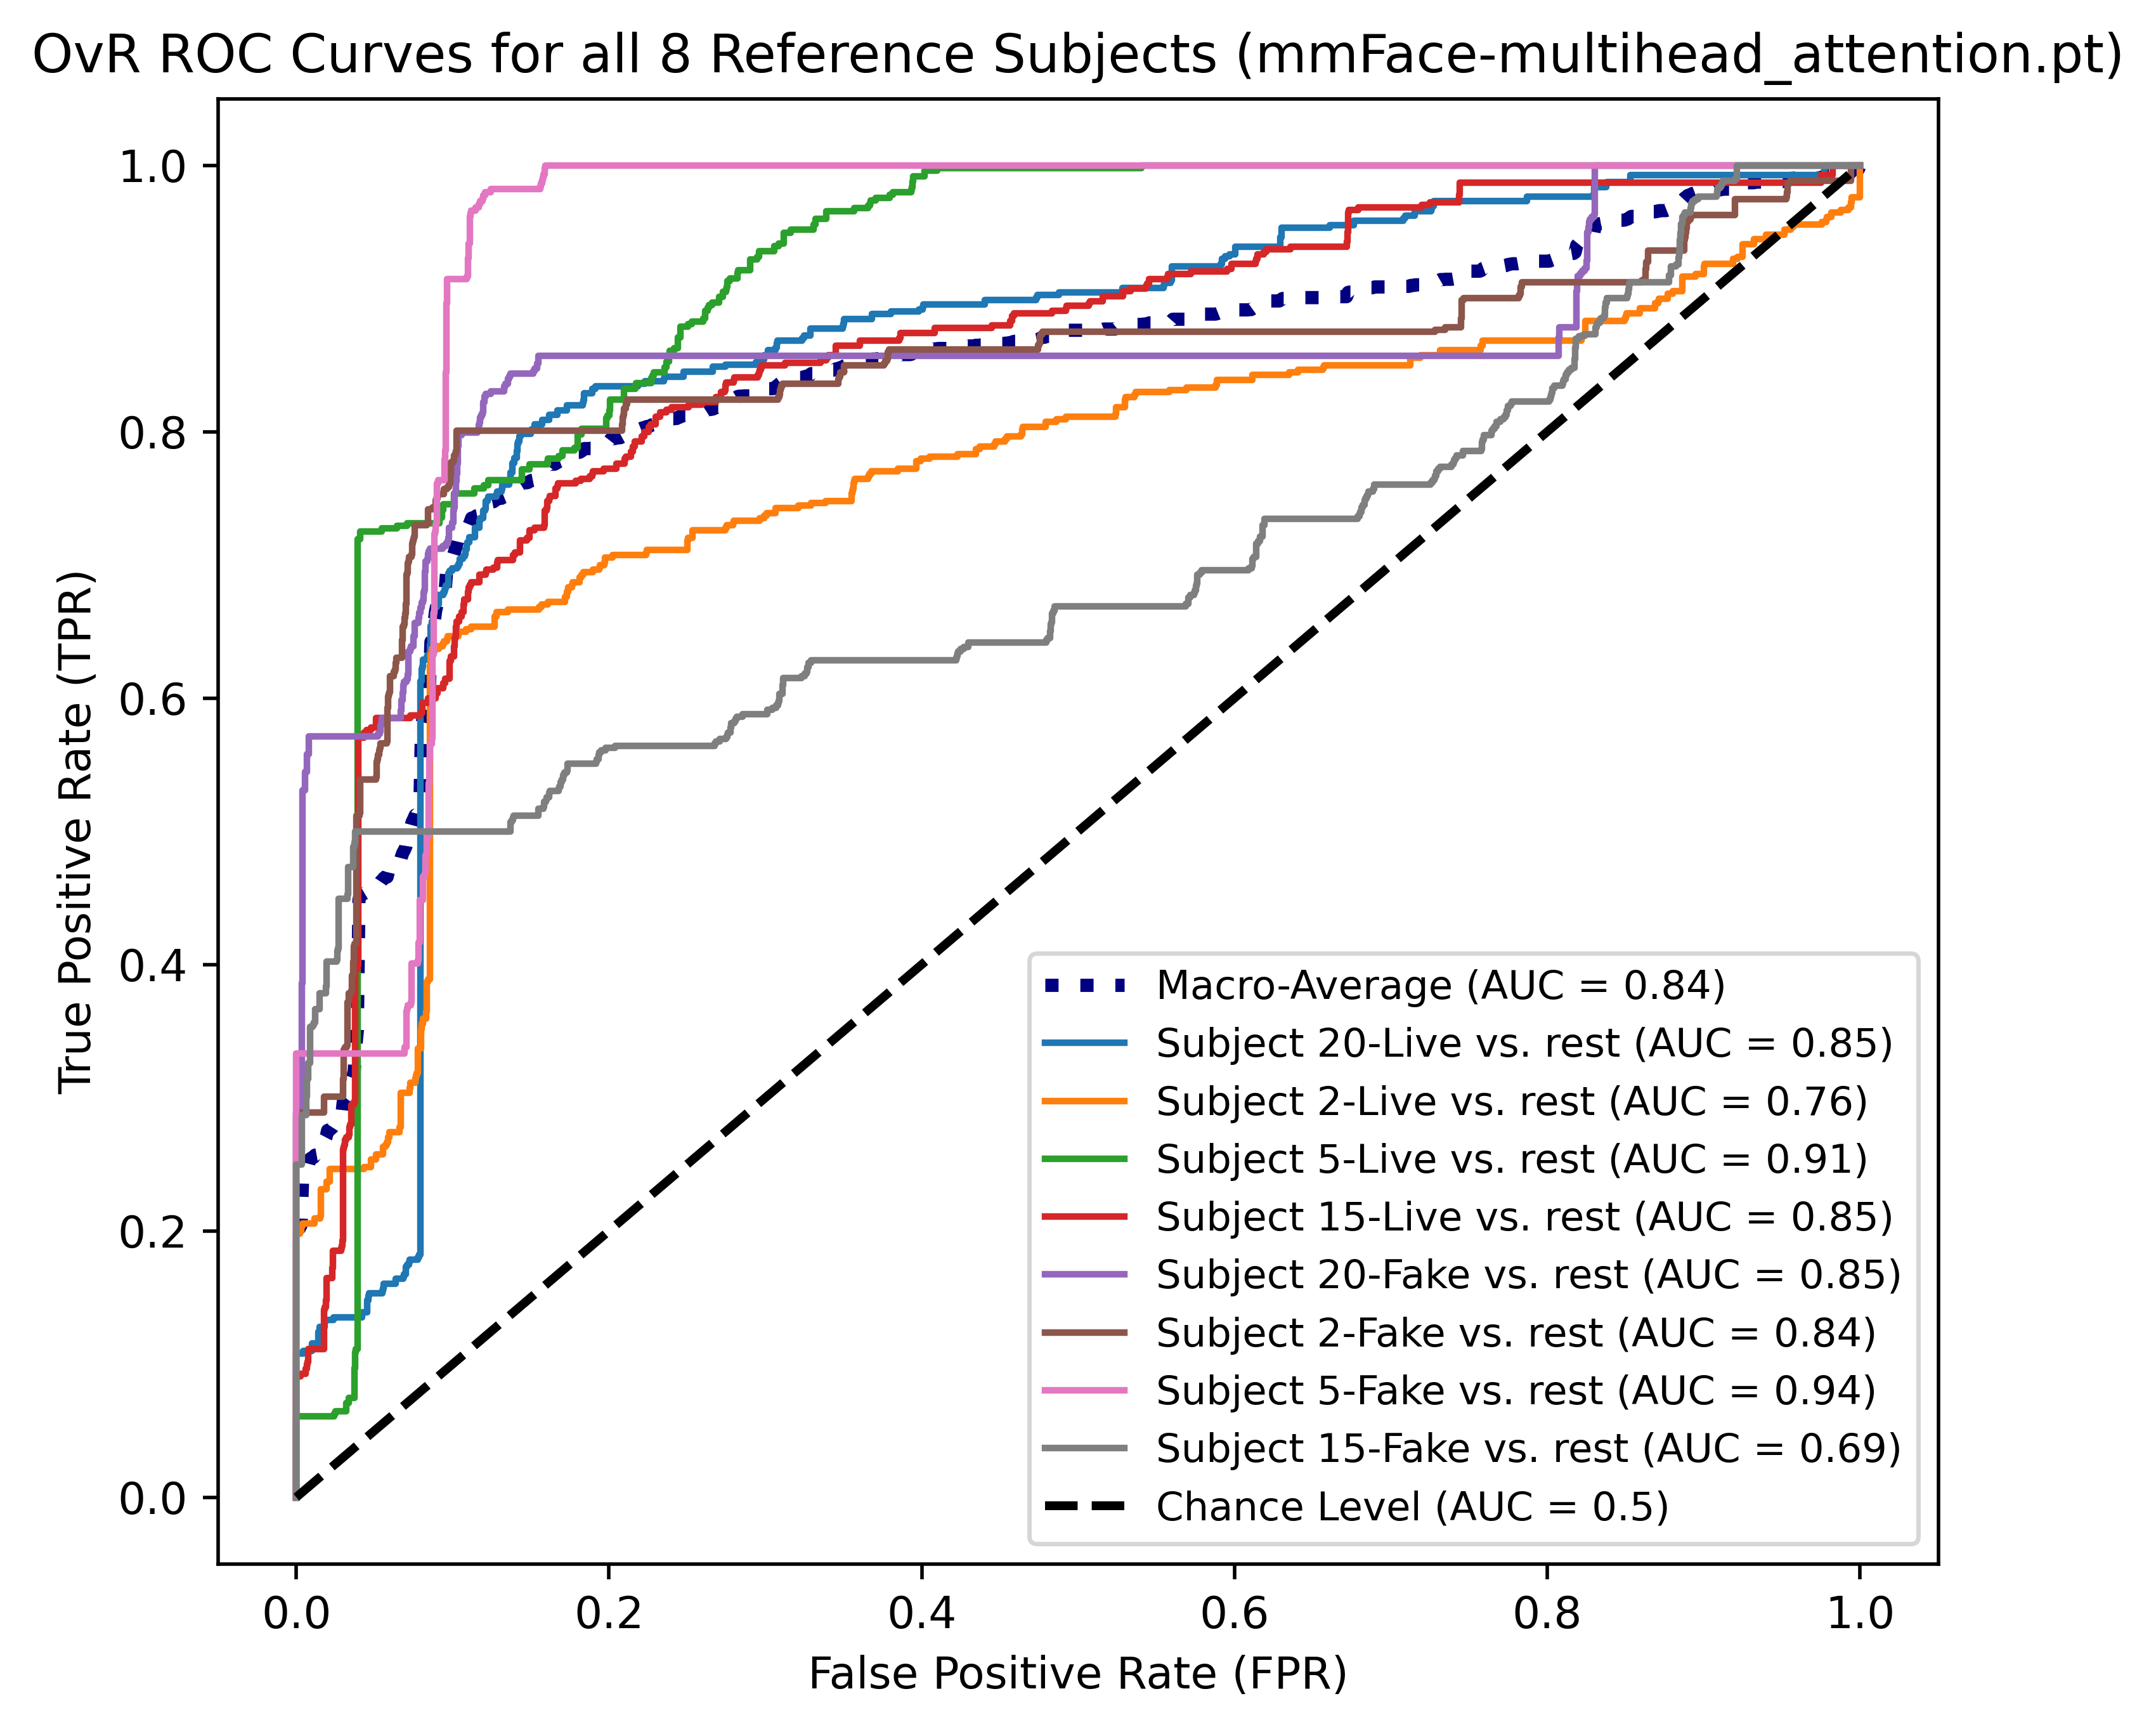
\includegraphics[width=\textwidth]{figures/roc_multihead_attention.png}
        \caption{Multi-Head Attention}
        \label{fig:roc_multihead_attention}
    \end{subfigure}
    \vspace{0.3cm}
    \caption{One-vs-the-Rest ROC curves plotted for each of the eight reference embeddings. Their respective AUC metrics are shown as well as the chance level and macro-averaged ROC curve.}
\end{figure*}

Table \ref{tab:macro_auc} lists the macro-averaged AUC metrics for all nine models. As made evident by the plot and the table, while the Hadamard product offers the highest accuracies it does not maintain its predictive nature across all decision thresholds attaining an AUC of 0.945. This is in contrast to the 0.961 AUC achieved by the concatenation strategy which ranked second-highest in overall performance. Figure \ref{fig:roc_concatenate} plots the one-vs-the-rest ROC curve for the concatenation approach. The plot shows that the concatenation performs equally well at distinguishing the majority of the reference instances since all curves are tightly packed and close to the top-left corner. In contrast, the ROC curves for the Hadamard product method are more dispersed with the relatively distinguishing ability for Subject 2-Live.
% TODO: SENSITIVITY & (1 - SPECIFICITY)
% TODO: ROC CURVE FOR MULTI-HEAD ATTENTION

It is important to note that the AUC metric is invariant to the decision threshold which has a profound impact whenever there is disparity in the cost of false negatives over false positives. In face recognition, especially for secure biometric authentication, false positives indicate a large flaw meaning the model should prioritise minimising them, even if that entails an increase of false negatives which are more tolerable. This is especially true for the binary liveness check. The model should be rewarded for minimising the success rate of 2D spoofing attacks.

\begin{table}[htbp]
    \centering
    \resizebox{0.8\columnwidth}{!}{
        \begin{tabular}{lcc}
            \toprule
            \textbf{Fusion Strategy}   & \textbf{Macro-Averaged AUC} \\
            \midrule
            \rowcolor{lightgreen}
            Concatenate          & 0.961 \\
            Add                  & 0.918 \\
            Hadamard Product     & 0.945 \\
            Pairwise Dot Mean    & 0.914 \\
            \rowcolor{lightred}
            Pairwise Dot Max     & 0.863 \\
            Pairwise Dot Flatten & 0.925 \\
            Multi-Head Attention & 0.913 \\
            \midrule
            Radar Only           & 0.735 \\
            RGB Only             & 0.901 \\
            \bottomrule
        \end{tabular}
    }
    \vspace{0.1cm}
    \caption{Table listing the macro-averaged AUC metrics for all fusion methods as well as the individual modalities.}
    \label{tab:macro_auc}
\end{table}


\subsubsection{t-SNE Visualisations}
Following this, it is important to visualise the final embedding vectors of each model to verify that each identity is pushed to distinct regions of the high-dimensional Euclidean space. $t$-distributed Stochastic Neighbour Embedding or $t$-SNE \cite{van2008visualizing} is commonly employed to reduce the dimensionality of the feature vectors to a lower space that can be easily visualised. t-SNE tends to preserve the local structure of the data much better in comparison to Principal Component Analysis (PCA) which is better at keeping the global variance in the data. This means that t-SNE can help identify meaningful patterns or groupings within the data since the similarities between data points are maintained providing interpretable visualisations.

Figures \ref{fig:tsne_hadamard_product}, \ref{fig:tsne_concatenate}, and \ref{fig:tsne_multihead_attention} show the final features of the top three ranking overall strategies after t-SNE, namely, the Hadamard product, concatenation, and multi-head attention approaches. Each data point is colour-coded by the subject identity with those coming from fake subjects having a lighter shade. It is clear that all three strategies group face data from the same subject into similar regions of the multimodal space. It can be observed that fusion by concatenation results in a tighter clustering with more separation between the distinct grouped islands of data points. Not only that, but it can be seen that some data points overlap with non-similar clusters in each of the strategies. This would entail lower subject identity accuracies with the least being observed within the Hadamard product, backed by its highest subject prediction accuracy out of the three. However, the concatenation strategy produces a clear linear separation between fake and real faces backing up the 99.6\% liveness detection accuracy. The other two strategies do not have such a clear separation, requiring more non-linear boundaries.

It is evident that there is more noise among the features from the real dataset compared to the fake, producing more distinct clusterings and confusion among all three strategies. This can be attributed to the higher level of variation of poses among the real dataset in contrast since only the frontal poses were utilised for the fake dataset. 

\begin{figure*}[!htb] 
    \centering
    \begin{subfigure}[b]{0.3\textwidth}
        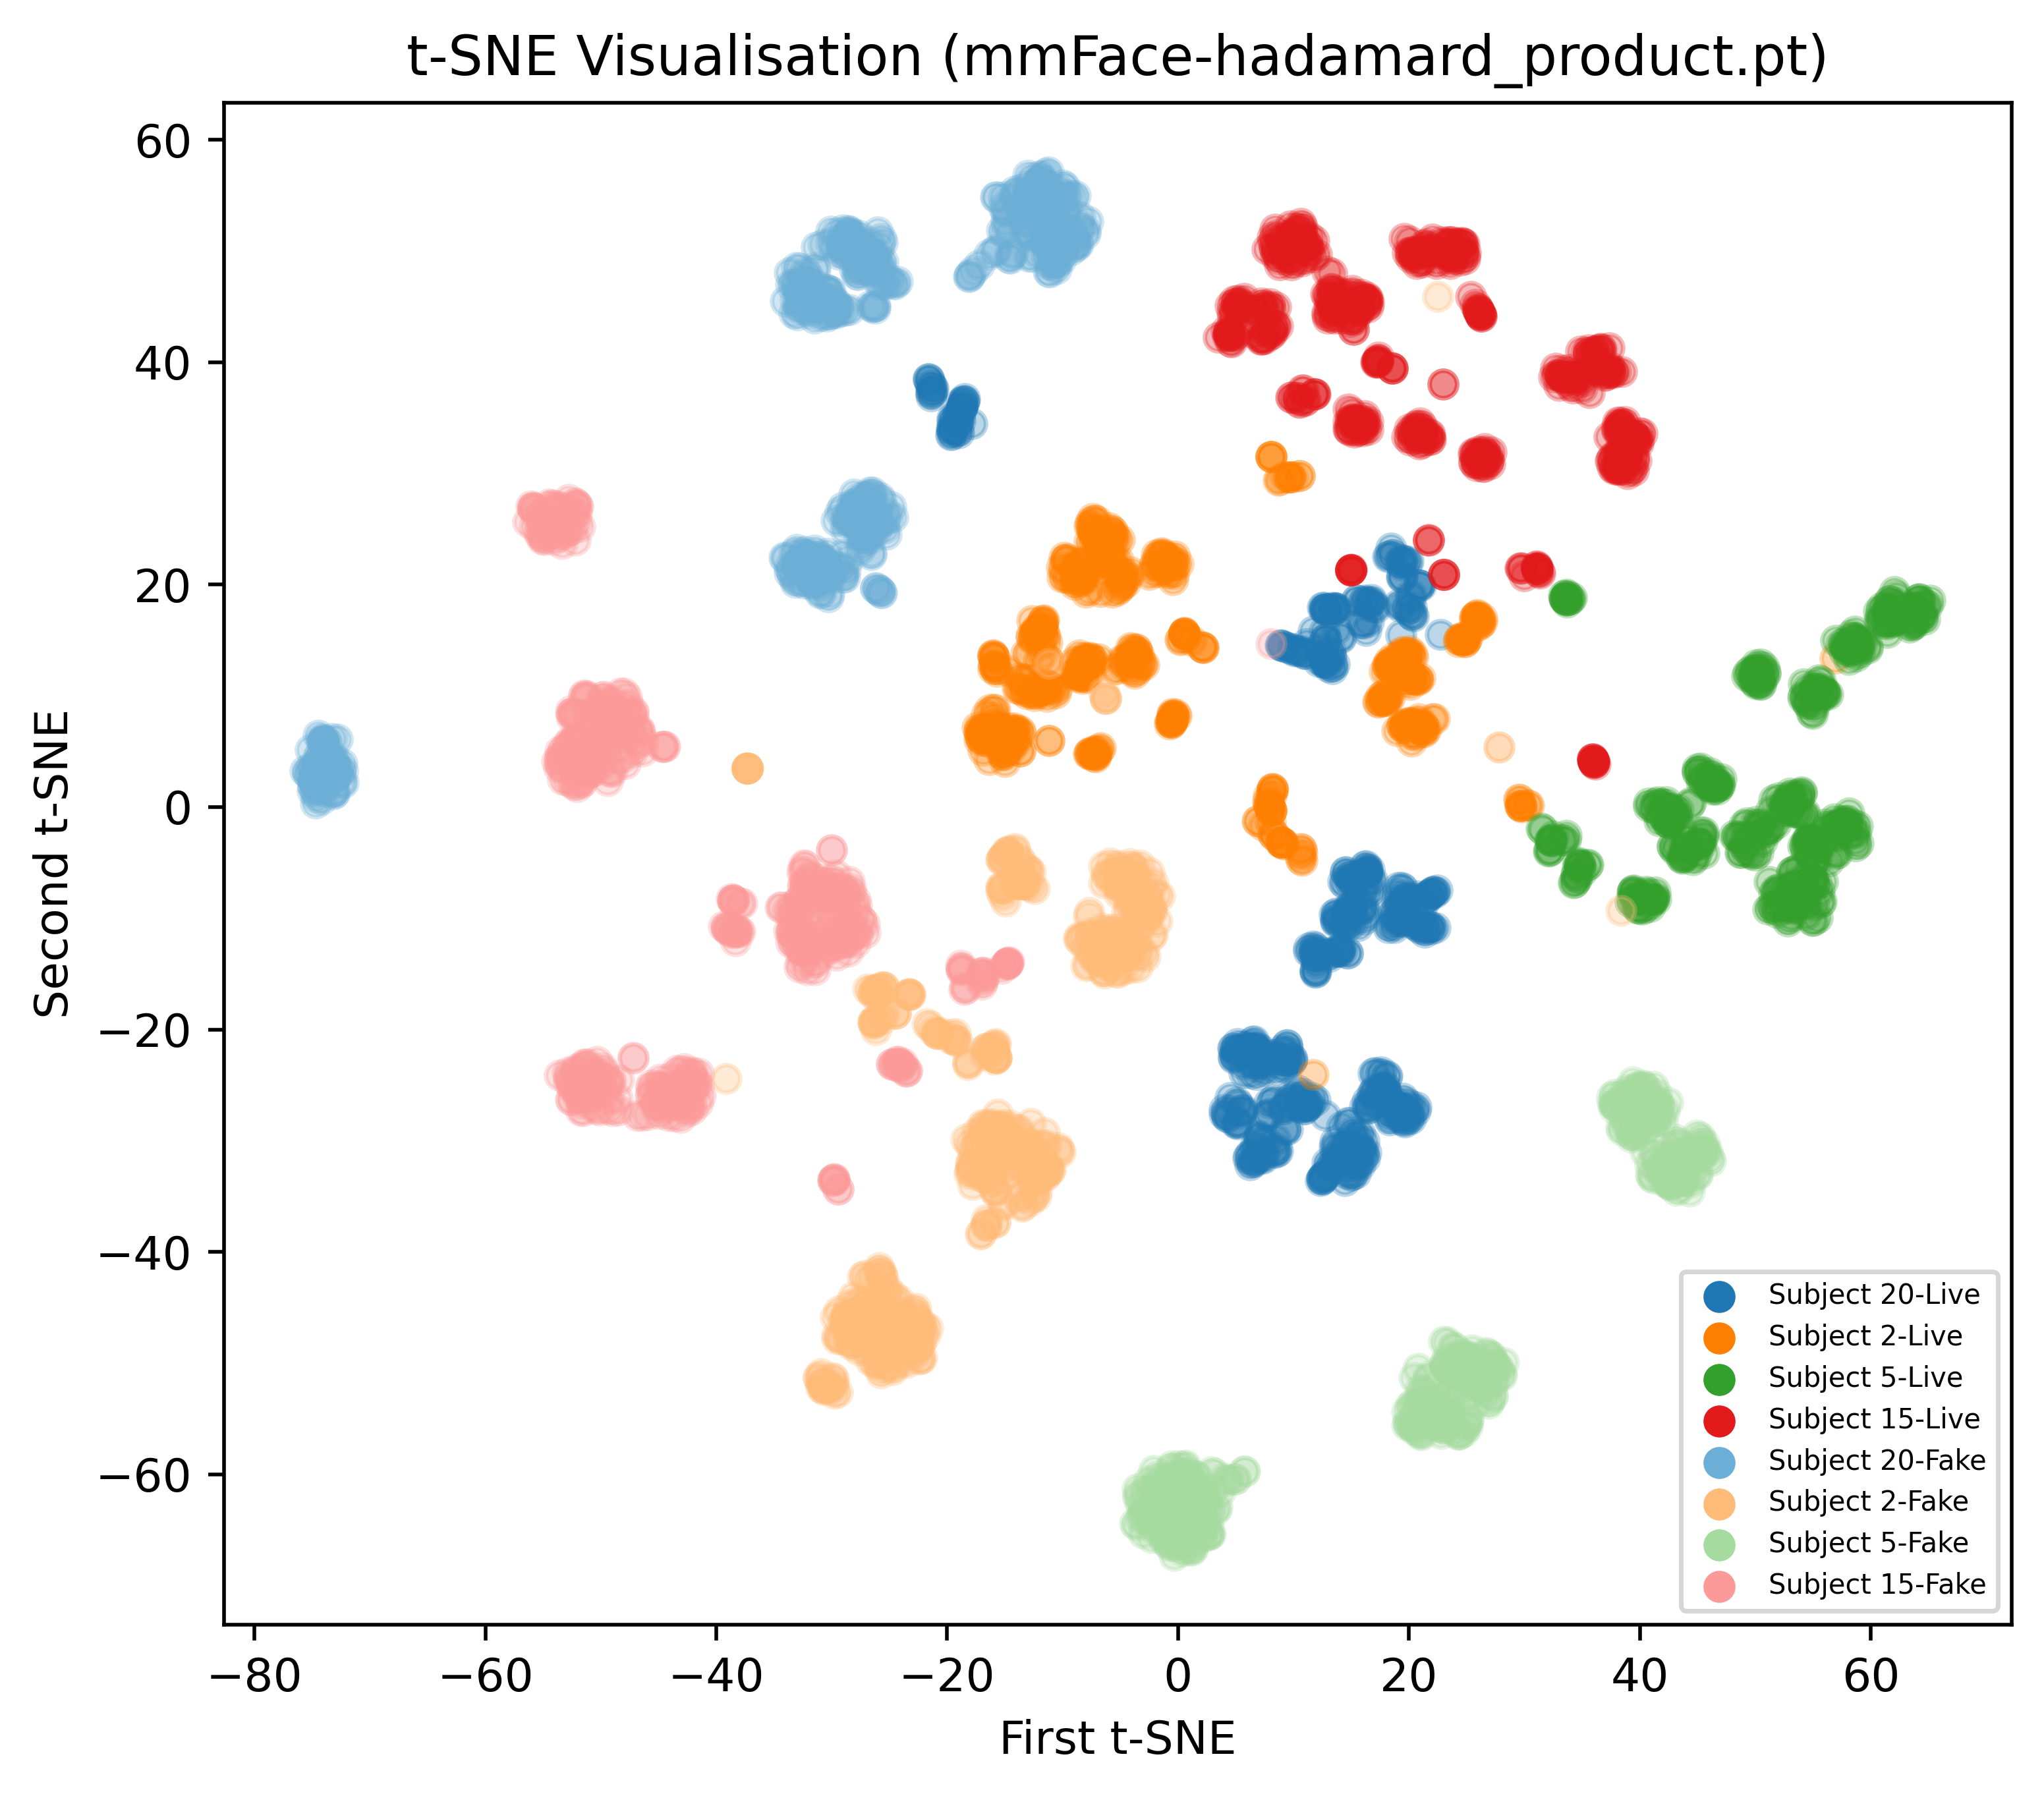
\includegraphics[width=\textwidth]{figures/tsne_hadamard_product.png}
        \caption{Hadamard Product}
        \label{fig:tsne_hadamard_product}
    \end{subfigure}
    ~
    \begin{subfigure}[b]{0.3\textwidth}
        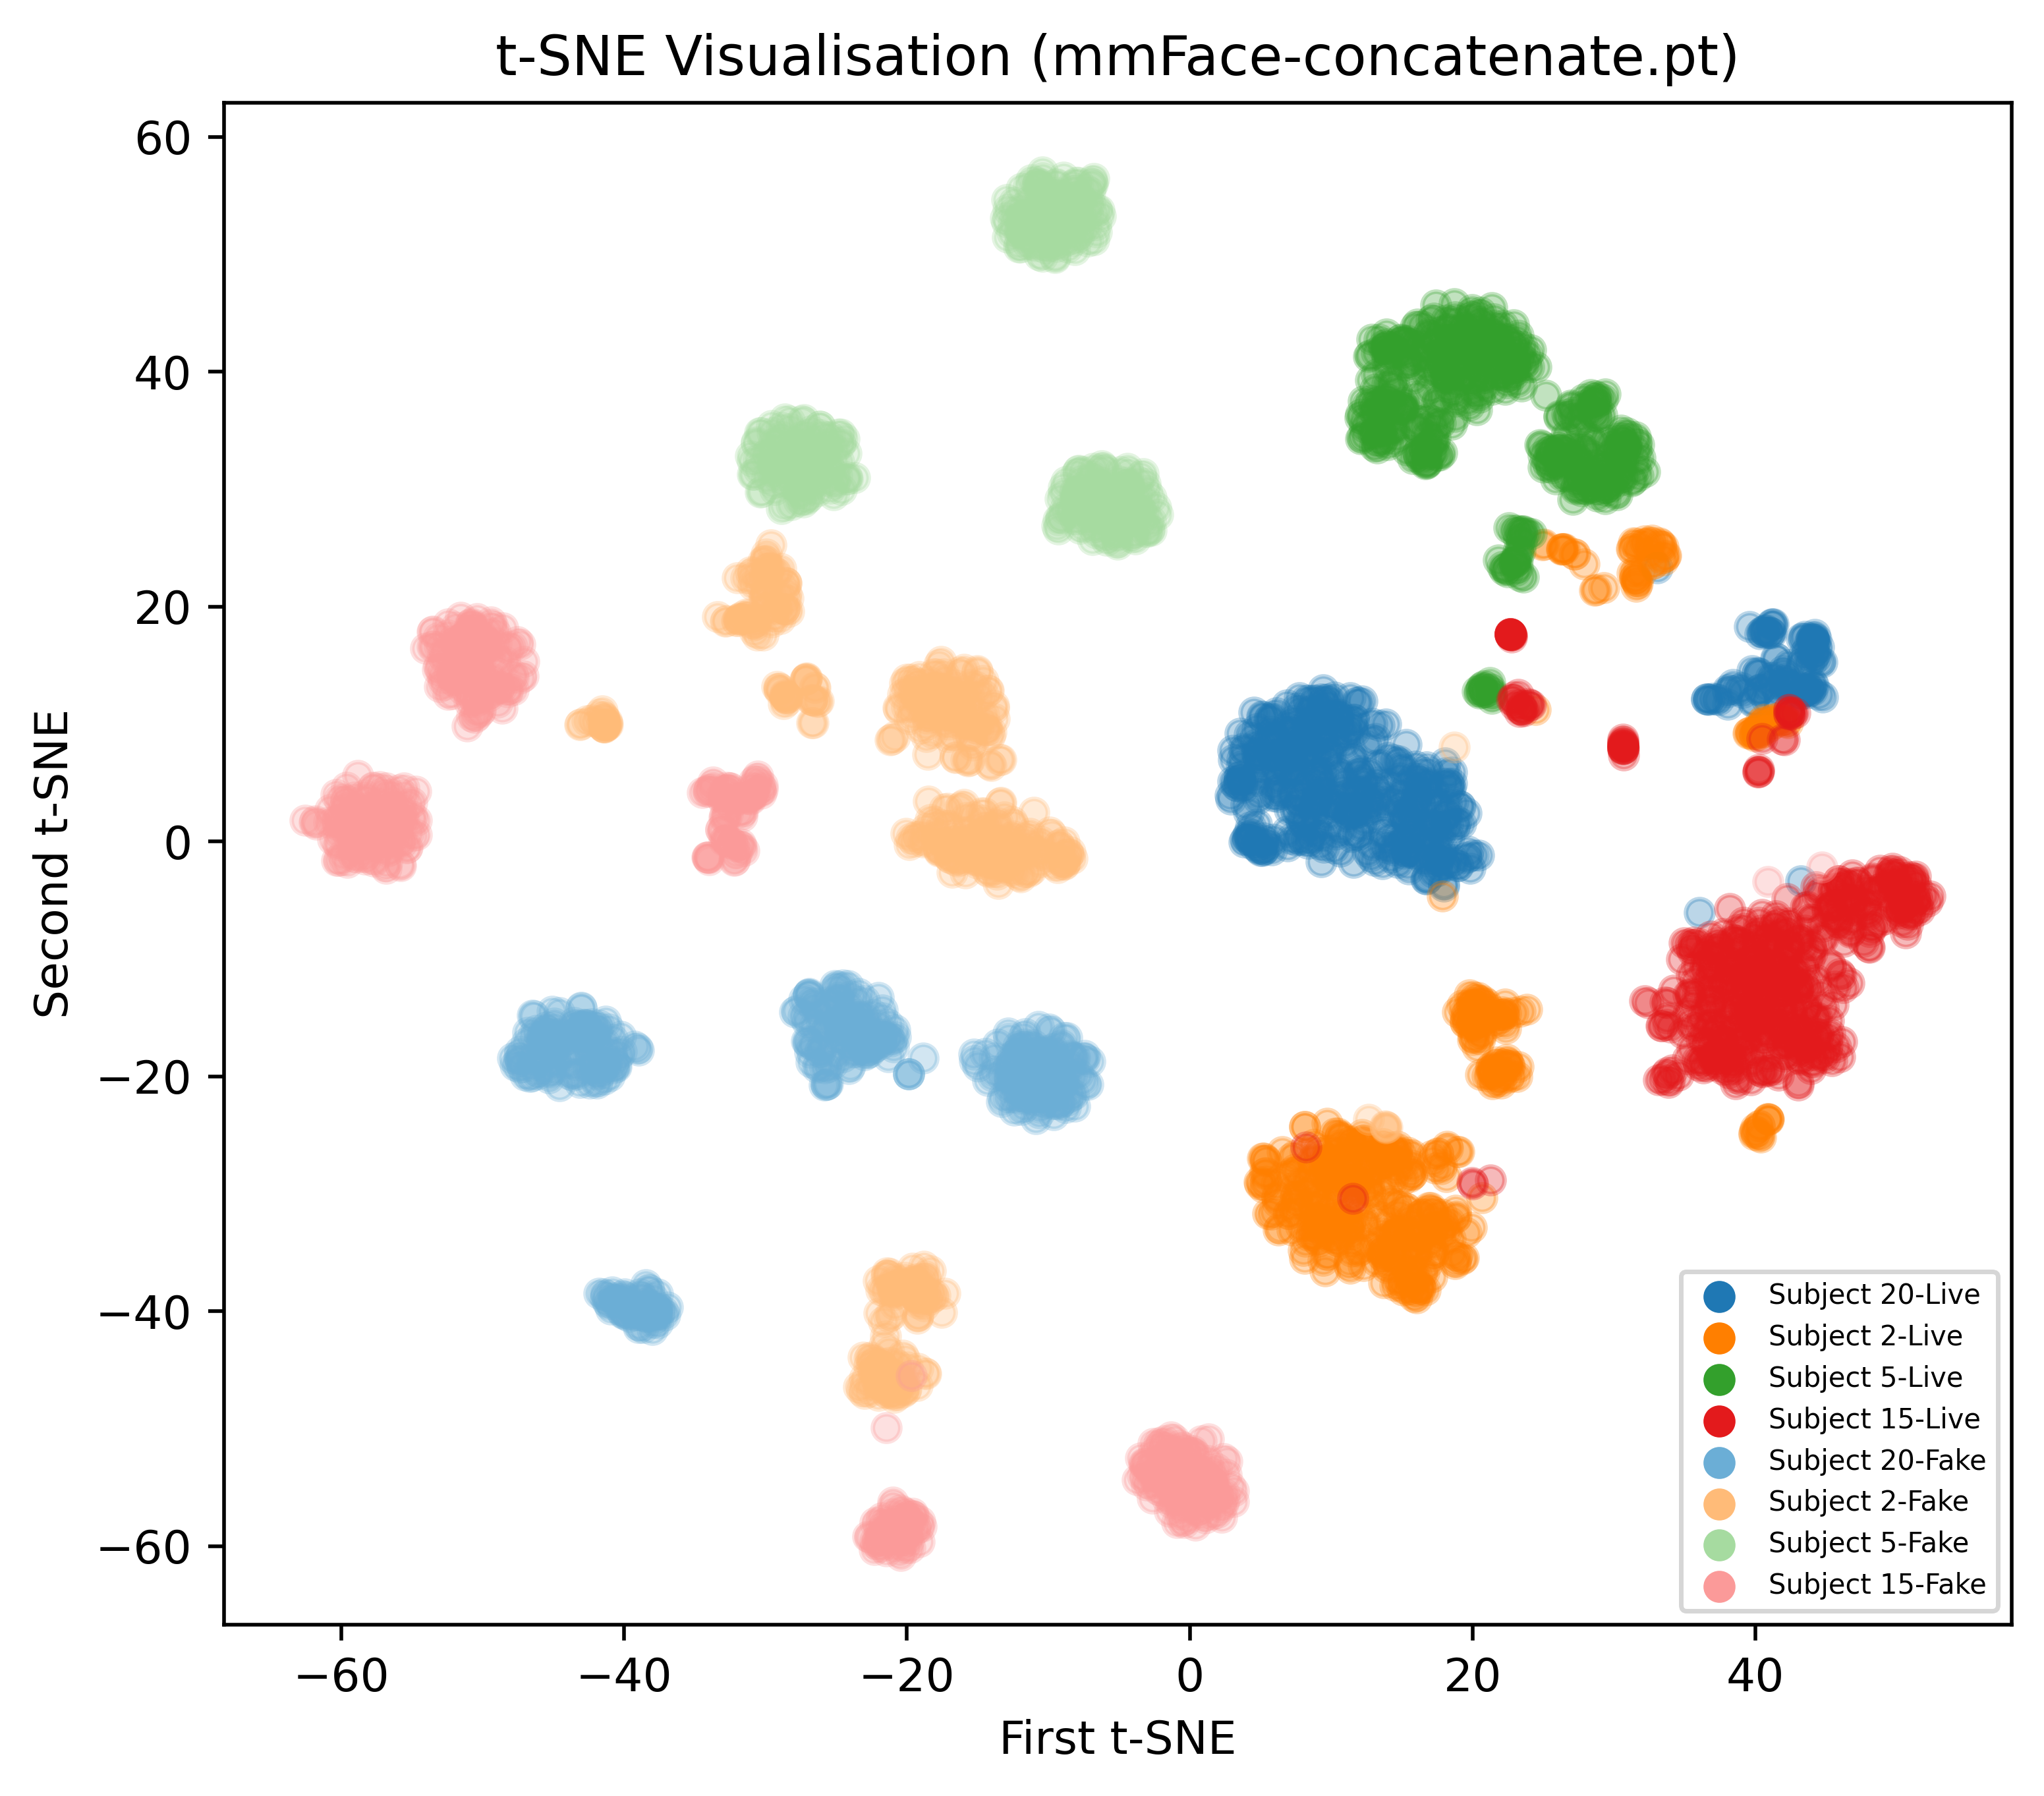
\includegraphics[width=\textwidth]{figures/tsne_concatenate.png}
        \caption{Concatenate}
        \label{fig:tsne_concatenate}
    \end{subfigure}
    ~
    \begin{subfigure}[b]{0.3\textwidth}
        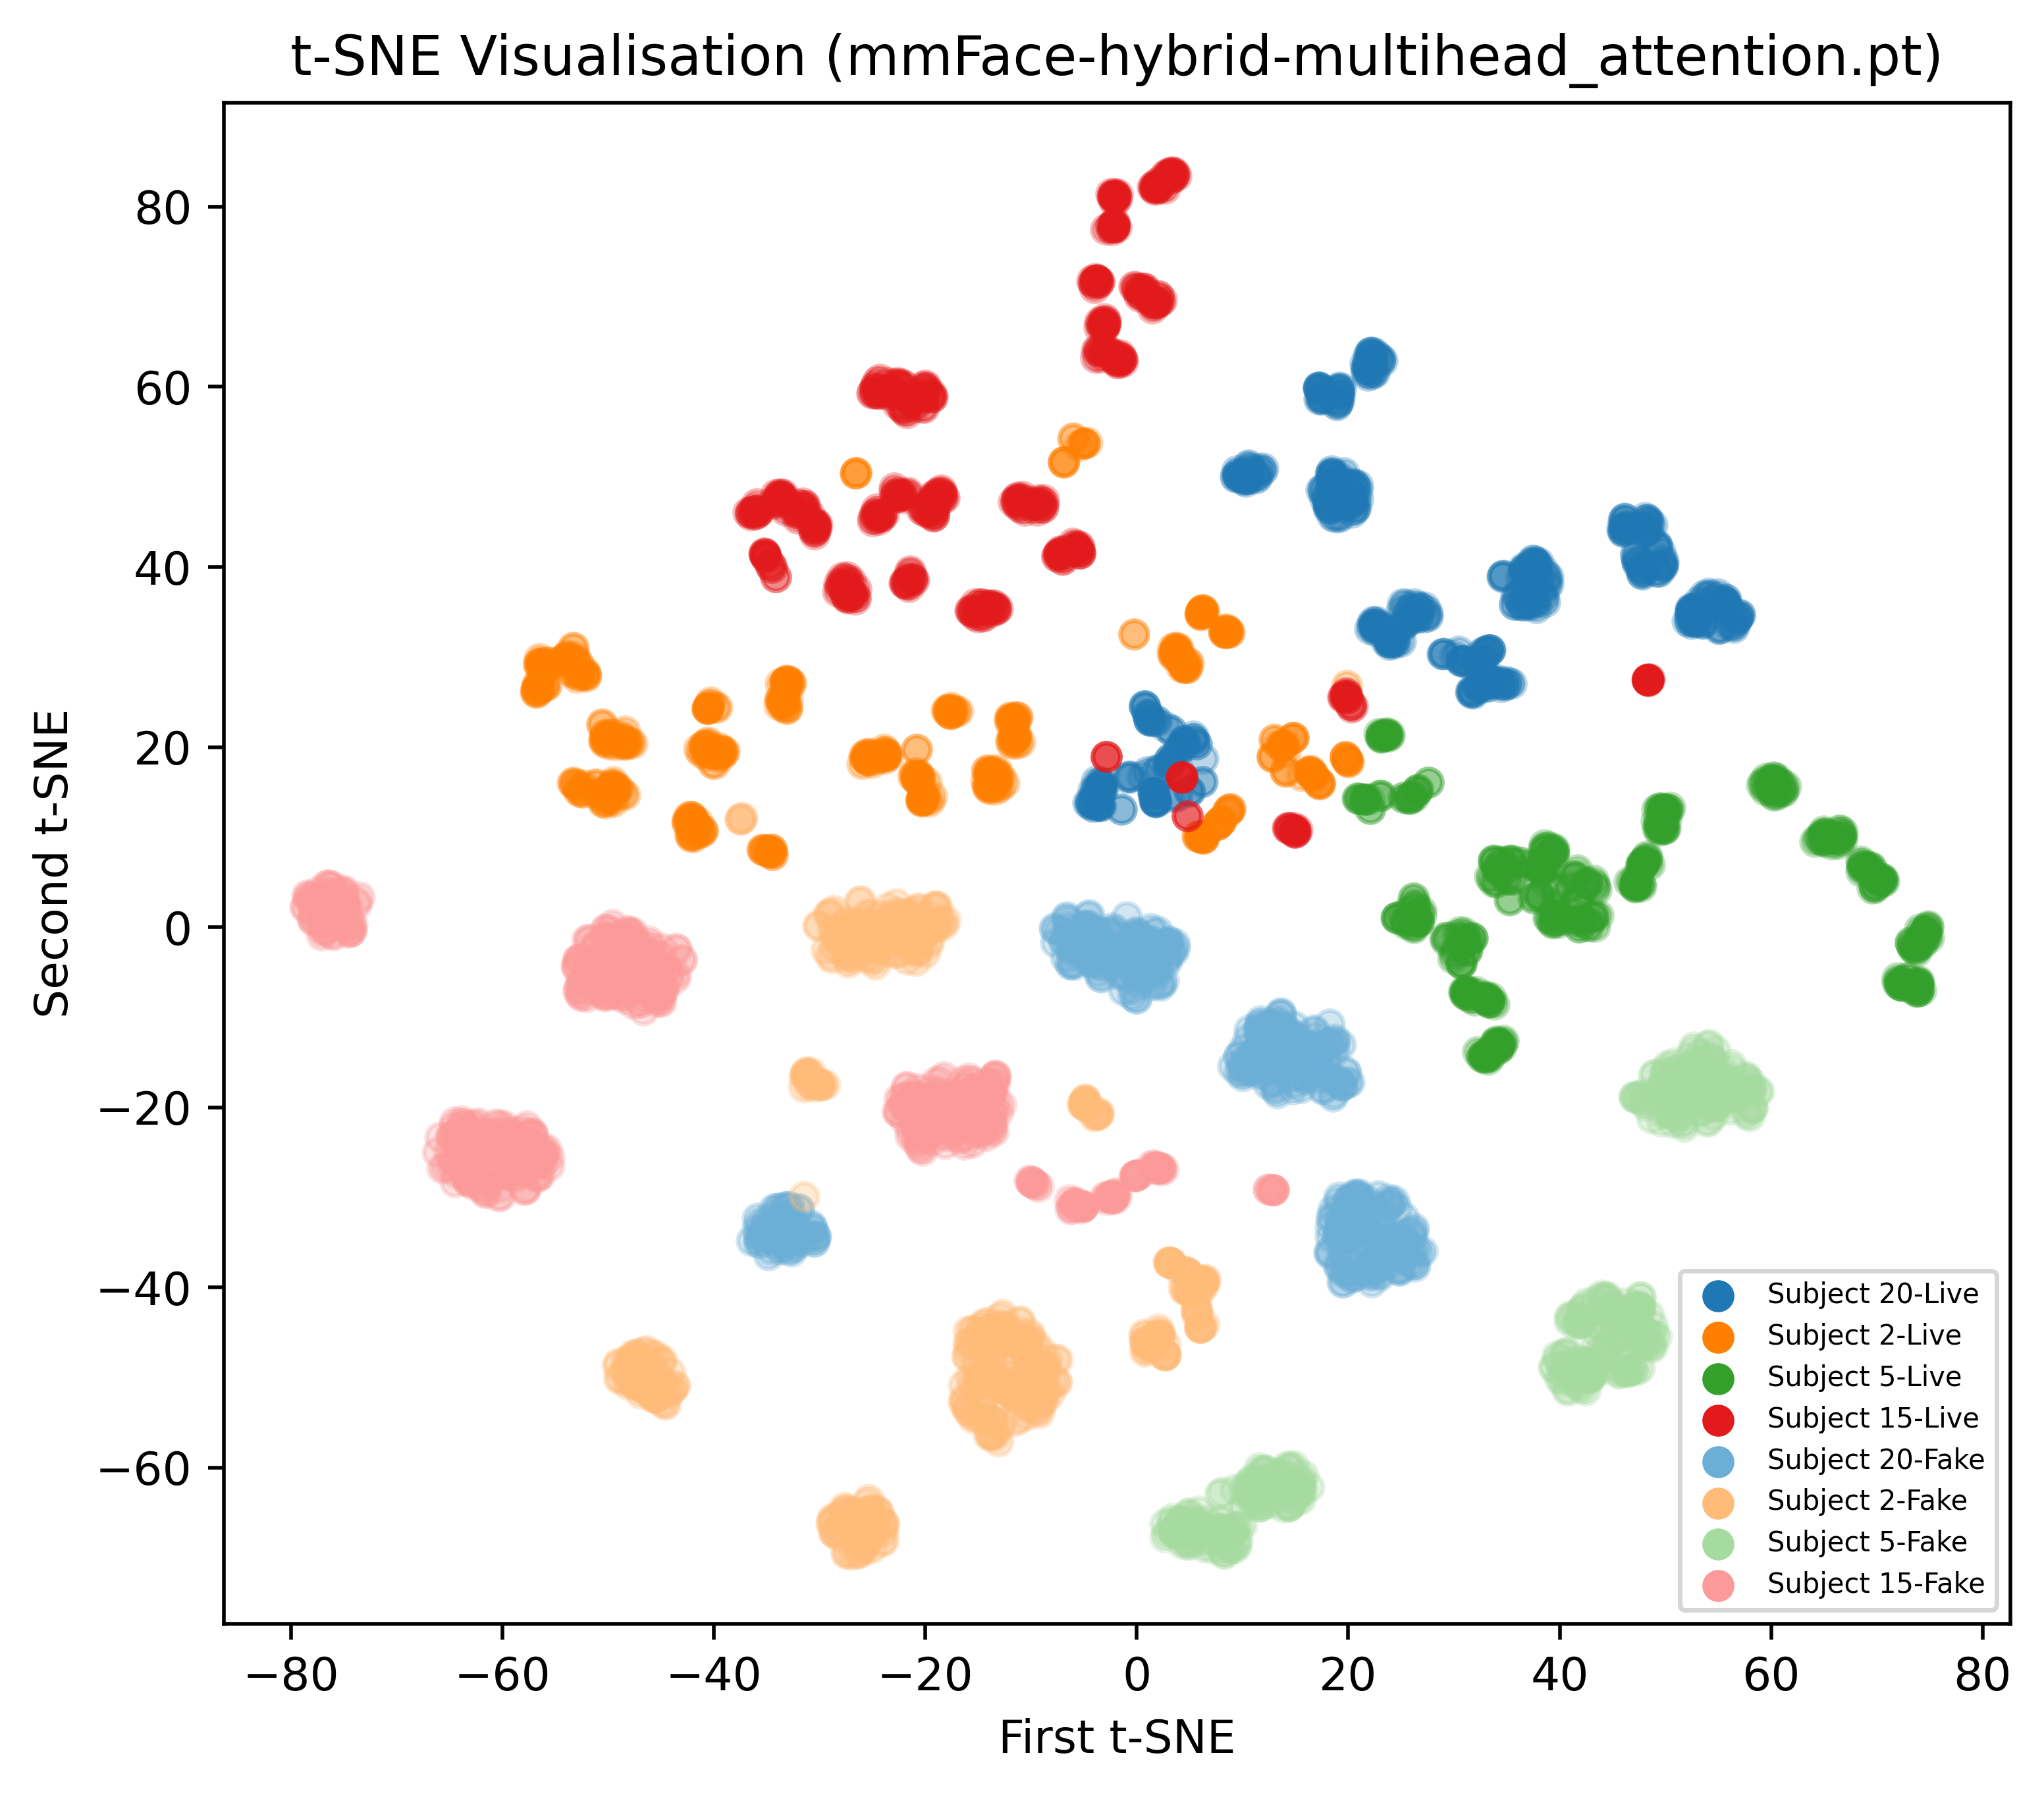
\includegraphics[width=\textwidth]{figures/tsne_multihead_attention.png}
        \caption{Multi-Head Attention}
        \label{fig:tsne_multihead_attention}
    \end{subfigure}
    \vspace{0.3cm}
    \caption{2D t-SNE projections of the final layer fused features after $\mathtt{fc\_hybrid1}$ of the model. Top three fusion strategies in the order of the highest overall mean accuracy.}
\end{figure*}

TODO: RESULTS OF DIM LIGHTING AND OCCLUSION SCENARIO



\section{Conclusions}



\subsection{Future Work}


{\bf Acknowledgments.}
This is optional; it is a location for you to thank people, most probably your family and your supervisor.


\bibliographystyle{unsrt}
\bibliography{l5proj}

\end{document}
